% -------------------------------
% == REPORT 3 ==
% -------------------------------

\documentclass[conf]{new-aiaa}

\usepackage[utf8]{inputenc}
\usepackage{float}
\usepackage{graphicx}
\usepackage{amsmath}
\usepackage[version=4]{mhchem}
\usepackage{siunitx}
\usepackage{longtable,tabularx}
\setlength\LTleft{0pt} 
\usepackage{hyperref}
\usepackage{nomencl}
\usepackage{lscape}

\linespread{2}  

\title{Design Report 03: Twin Sea Lion}

\author{
    Madison Junker\footnote{Student ID: 102736535 }, Jacob Killelea\footnote{Student ID: 10550162 } \\
    \emph{ASEN 4138, University of Colorado Boulder, November 16, 2018}
}

\begin{document}

\clearpage
\maketitle
\thispagestyle{empty}

\newpage
\pagenumbering{roman}
\tableofcontents
\addcontentsline{toc}{section}{\listfigurename}
\listoffigures
\addcontentsline{toc}{section}{\listtablename}
\listoftables
\newpage
\printnomenclature[25mm]

\section*{Nomenclature}

{\renewcommand\arraystretch{1.0}
\noindent\begin{longtable*}{@{}l @{\quad=\quad} l@{}}
$AAA$     	               & Advanced Aircraft Analysis Program \\
$AR_W$    	               & Wing Aspect Ratio          \\
$b_W$	  	               & Wing Span                  \\
$b_h$	  	               & Horizontal Stabilizer Span \\
$b_v$	  	               & Verctial Stabilizer Span   \\
$b_e$	  	               & Elevator Span   \\
$b_r$	  	               & Rudder Span   \\
$\bar{c}_W$	  	           & Mean Geometric Chord               \\
$CG$	  	               & Center of Gravity \\
$ft$	  	               & Feet \\
$i_W$		               & Incidence Angle                    \\
KTAS                       & Knots True Airspeed                \\
$l_f$     	               & Length of fuselage                 \\
$\epsilon_W$               & Wing Twist Angle                   \\
$\eta_{a_i}$               & Aileron Inboard Station as Fraction of Half-Span \\
$\eta_{a_0}$               & Aileron Outboard Station as Fraction of Half-Span \\
$\Lambda_{c/4w}$[$^\circ$] & Wing Sweep Angle                   \\
$\lambda_W$	               & Wing Taper Ratio                        \\
$\lambda_h$	               & Horizontal Stabilizer Taper Ratio                        \\
$\lambda_v$	               & Vertical Stabilizer Taper Ratio                        \\
$\lambda_{c/4w}$           & Quarter-chord Sweep Angle          \\
$lbs$                      & Pounds Mass \\
$M$                        & Mach Number \\
$MSL$     	               & Mean Sea Level Altitude            \\
$NACA$                     & National Advisory Committe for Aeronautics \\
$S_W$     	               & Wing Area                          \\
$S_h$     	               & Horizontal Stabilizer Area \\
$S_v$     	               & Vertical Stabilizer Area  \\
$S_e$     	               & Elevator Area  \\
$S_r$     	               & Rudder Area  \\
$TWR$     	               & Thrust to Weight Ratio             \\
$V_h$     	               & Horizontal Tail Volume Ratio \\
$V_v$     	               & Vertical Tail Volume Ratio \\
$\Gamma_W$	               & Dihedral                           \\
$W_{lav}$	               & Lavatory Weight                           \\
$x_{cg}$	               & X Location of the Center of Gravity \\
$y_{cg}$	               & Y Location of the Center of Gravity \\
$z_{cg}$	               & Z Location of the Center of Gravity \\
\end{longtable*}}

\newpage
\pagenumbering{arabic}

% 1
\section{Introduction}
In this report, the Sea Lion gets the weight and $c_g$ of each major component defined in order to develop a loading order that will not tip over the plane. Defining the plane's $c_g$ also allows empennage design and stability characterization. 

\section{Preliminary Weight and Balance Analysis}

\subsection{Preliminary Weight Breakdown}
%Define/show axis system

The very nose of the plane defines x axis zero, the plane of symmetry of the plane defines y axis zero with the right wing going in the positive y direction, and the bottom of the wing defines z axis zero with positive z going upwards.

% Explain the empty weight breakdown of your aircraft, including individual 
%adjusting weight groups
Propeller diameter was determined from the Gerren equation as included below\cite{pres18}. Above 4 blades, $K_p$ is not explicitly defined, so $K_p=1.1$ was assumed to account for the 8 blades used. This results in $D=1.1(5000)^{1/4}=9.25$ ft.

\[ D = K_p(\frac{Power}{Engine})^{1/4} \ \ where\ \ \begin{cases} 
      Blades & K_p \\
      2 & 1.7 \\
      3 &  1.6 \\
      4+ & 1.5 
   \end{cases}
\] 

From AAA figure \ref{fig:propellerweight}, propellers with a 9.25 foot diameter will weigh about 1800 lbs. The engines themselves weigh 3000 lbs and about 700 lbs of extra power plant weight was added to account for additional powerplant needs. This number was reduced from normal extra engine weight by the use of electronic actuators. Total powerplant weight is about 5500 lbs. The initial weight breakdown in figure \ref{fig:weightfractionsinitial} gave 4627.2 lbs for powerplant, so some extra weight for the engines had to be found by downsizing other components. 

Figure \ref{fig:weightfractionsfinal} shows the final weight breakdown obtained by moving the initial weight fractions obtained from similar airplanes to a single custom airplane shown in figure \ref{fig:customairplane} and basing the new estimate solely on that custom airplane. The wing weight fraction was reduced from 0.107 to 0.095, which will be done through the use of composite materials. This same method will allow the reduction of empennage weight fraction from 0.027 to 0.020. 

These changes allowed an increase in powerplant weight fraction from 0.127 to 0.157 and also allowed an increase in gear weight fraction from 0.042 to 0.046. Powerplant weight budget increased to 5596.2 lbs, which is now sufficient to account for engines, propellers, and extra powerplant weight.

%Empty weight breakdown
These final weights were used to obtain an empty weight breakdown as in table \ref{tab:Empty Weight}.

\begin{table}[H]
\centering
\label{tab:Empty Weight}
\caption{Empty weight breakdown of the Sea Lion.}
\begin{tabular}{|c|c|c|c|c|c|c|}\hline
Fuselage & Wing & Empennage & Landing Gear & Nacelle & Powerplant & Fixed Equipment \\ \hline
4455.5 & 3386.2 & 712.9 & 1639.6 & 855.5 & 5596.2 & 5275.4 \\ \hline
\end{tabular}
\end{table}
% tables with structural, powerplant, and fixed equipment weight breakdowns
The structural weight breakdown is based on the empty weight breakdown but separates empennage into vertical and horizontal tails and gear into nose and main gear. Vertical tail weight was assumed to be 3/8 of allotted tail weight to approximately conform to Beech 1900 tail area proportions as in table 8.6 of the technical documentation\cite{orange_book}. So the vertical tail weighs $\frac{3}{8}712.9=267.3$ lbs and the horizontal tail weighs $712.9-267.3=445.6$ lbs. 

Nose gear was assumed to be 15\%\cite{pres19} of the gear weight at $0.15\cdot1639.6=245.9$ lbs with the main gear taking the remaining weight of $1639.6-245.9=1399.7$. 
\begin{table}[H]
\centering
\label{tab:Structural Weight}
\caption{Structural weight breakdown.}
\begin{tabular}{|c|c|c|c|c|c|}\hline
Wing & Fuselage & Horizontal Tail & Vertical Tail & Nose Gear & Main Gear \\ \hline
3386.2 & 4455.6 & 445.6 & 267.3 & 245.9 & 1399.7 \\ \hline
\end{tabular}
\end{table}

Power plant weight was determined by dividing the allowed weight in two and subtracting the 901.8 allotted for each side of propeller.

\begin{table}[H]
\centering
\label{tab:Powerplant Weight}
\caption{Powerplant weight breakdown.}
\begin{tabular}{|c|c|c|c|}\hline
Engine 1 & Engine 2 & Propeller 1 & Propeller 2 \\ \hline
1896.3 & 1896.3 & 901.8 & 901.8 \\ \hline
\end{tabular}
\end{table}

Weight of the lavatory is determined as follows $W_{lav} = K_{lav}(N_{pax})^1.33=3.9(10^{1.33})=83.38$lbs\cite{pres19}. $K_{lav}$ of a business jet was chosen to account for this equation's tendency to underestimate the weight of the lavatory.

\begin{table}[H]
\centering
\label{tab:Fixed Equipment Weight}
\caption{Fixed equipment $c_g$}
\begin{tabular}{|c|c|}\hline
Lavatory & Other \\ \hline
83.4 & 5192.0 \\ \hline
\end{tabular}
\end{table}
% and the x-,y-, and z-cg locations of the various weight components. You can

With the wing apex at 21 feet, the $x_{cg}$ was places two feet behind the apex. Since the wing is symmetric across the y axis, $y_{cg}=0$. With a 12\% thick airfoil and a root chord of 12.79 ft, the maximum thickness of the wing will be 1.53 feet. Half this width plus a little more than a foot from the bottom of the airplane to the bottom of the wing gives $z_{cg}=2$ feet.

Fuselage $x_{cg}$ was approximated at 0.45 of length\cite{pres19} to be $0.45\cdot47.58=21.41$ ft.

Approximate landing gear dimensions from table 9.1 of the landing gear technical documentation\citet{orange_book} give a main gear tire width of 9 inches and a nose gear tire diameter of 23.4 inches. The z direction offset will be 4.5 inches for the main gear and 11.7 inches for the nose gear. These correspond to 0.98 ft in the z direction for the nose gear and $2+\frac{4.5}{12}=2.38$ ft for the main gear.

All structural components are symmetric about the y axis.
\begin{table}[H]
\centering
\label{tab:Structural cg}
\caption{Structural $c_g$ breakdown.}
\begin{tabular}{|c|c|c|c|}\hline
	& $x_{cg}$ [ft] & $y_{cg}$ [ft] & $z_{cg}$ [ft] \\ \hline
Wing & 23 & 0 & 2\\ \hline
Fuselage & 21.41 & 0 & 3.5\\ \hline
Horizontal Tail & 62 & 0 & 6\\ \hline
Vertical Tail & 62	& 0 & 16\\ \hline
Nose Gear & 8 & 0 & 0.98\\ \hline
Main Gear & 30 & 0 & 2.38\\ \hline 
\end{tabular}
\end{table}


The engines are 7.9 feet long and so suggest about 10 foot long nacelles. A suggested value of 0.4 the length of the nacelle \cite{pres19} puts the $x_{cg}$ of the engine 4 feet behind the beginning of the nacelle. Assuming the nacelle begins 1 ft ahead of the wing, the engine cg will be 3 ft behind the beginning of wing. Due to all the wing shifting that occurred in the stability adjustment, the engine cg ended up only 2 ft behind the beginning of the wing at 23 ft. 

The nacelles were assumed to be placed about 1 ft above the wing, making $z_{cg} = 3$. The propeller and fuselage radii require the engine to be 9 feet along the y axis to account for room taken up and some space in between: $\frac{82.5}{2\cdot12}+\frac{9.25}{2}=8.06$. One engine will be along the positive axis and the other the negative axis.

Propeller $x_{cg}$ will be about 1 ft ahead of the apex of the wing at 20 ft and will be at the same points in the y and z axes.

\begin{table}[H]
\centering
\label{tab:Powerplant cg}
\caption{Powerplant $c_g$ breakdown.}
\begin{tabular}{|c|c|c|c|}\hline
	& $x_{cg}$ [ft] & $y_{cg}$ [ft] & $z_{cg}$ [ft] \\ \hline
Engine 1 & 23 & 9 & 3\\ \hline
Engine 2 & 23 & -9 & 3\\ \hline
Propeller 1 & 20 & 9 & 3 \\ \hline
Propeller 2 & 20 & -9 & 3\\ \hline
\end{tabular}
\end{table}

Assuming the lavatory to be a rectangular prism of constant density, the solidworks model can be used to find the $c_g$ in any direction. The distance from the front of the plane to the middle of the lavatory is 499.5 inches. The distance from the centerline of the plane to the middle of the lavatory is 23.5 in. The distance from the bottommost part of the fuselage to the middle of the lavatory is 50.5 in.

\begin{table}[H]
\centering
\label{tab:Fixed equipment cg}
\caption{Fixed equipment $c_g$ breakdown.}
\begin{tabular}{|c|c|c|c|}\hline
	& $x_{cg}$ [ft] & $y_{cg}$ [ft] & $z_{cg}$ [ft] \\ \hline
Lavatory & 41.63 & 1.96 & 4.21\\ \hline
Other & 21.41 & 0 & 3.5\\ \hline

\end{tabular}
\end{table}


\subsection{Preliminary Weight and Balance Calculation}
%Explain the fully-loaded weight breakdown of your aircraft, including a table with the loaded component weights and x-,y- and z-cg locations. Again, you can "cut and paste" as above.
%Include the loading scenario. Explain how you grouped things (like passengers, munitions, etc.) and determined the order in which items are loaded/unloaded. Show the X-cg and Z-cg excursion plots.
%List the fully-loaded, forward and aft cg locations (need X and Z values for each). Calculated your X-cg shift from most forward to most aft location, and divide by your mean aerodynamic chord. Compare you values (in inches as well as divided by c) with those in Tables 10.3 of c (posted on Canvas under Technical Documentation).

\begin{table}[H]
\centering
\label{tab:weight and cg fully loaded}
\caption{Fully-loaded weight and $c_g$ breakdown.}
\begin{tabular}{|c|c|c|c|c|}\hline
						& Weight [lb] & $x_{cg}$ [ft] & $y_{cg}$ [ft] & $z_{cg}$ [ft]\\ \hline
Crew 					& 525 & 12.05 & -0.56 & 5\\ \hline
Trapped Fuel and Oil 	& 188.4 & 21.41 & 0 & 3.5\\ \hline
Mission Fuel Group 1 	& 10679.3 & 22 & 0 & 2\\ \hline
Passenger Group 1 		& 1750 & 28.92 & 0 & 5\\ \hline
Baggage 				& 605 & 28.92 & 0 & 3\\ \hline
Cargo 					& 2020 & 33 & -2 & 0\\ \hline

\end{tabular}

\end{table}

The most forward cg is 23.67 ft and the most aft cg is 24.78 ft. The total shift is 1.11 ft or 13.31 inches. The mean aerodynamic chord is 10.4 ft as follows\cite{aircraft dynamics}. The shift in $c_g$ as a portion of aerodynamic chord is $\frac{1.11\ ft}{10.4\ ft}=0.106=10.6\%$. From technical documentation, \cite{roskam 3} regional turboprops exhibit a typical $\Delta c_g=[12,20]$ with a proportion of mean aerodynamic chord of $\frac{\Delta c_g}{\bar{c}}=[0.14,0.27]$. The Twin Sea Lion falls in the range of $\Delta c_g$ and below the range of $\frac{\Delta c_g}{\bar{c}}$. This indicates that our change in $c_g$ is in the range of typical even though our wing is larger relative to this change than typical. 

\begin{equation*}
\bar{c}=\frac{2c_r}{3}\frac{1+\lambda+\lambda^2}{1+\lambda}=\frac{2(12.79\ ft)}{3}\frac{1+0.6+0.6^2}{1+0.6}=10.4\ ft
\end{equation*}



\begin{table}
\centering
\label{tab:Cg excursion ordering}
\caption{Cg excursion ordering.}
\begin{tabular}{|c|c|c|c|c|}\hline
			& Weight 	& $x_{cg}$ [ft] & Load & Unload \\ \hline
Empty Weight & 21921.3 & 23.96 & 1 & 13 \\ \hline
Crew & 525.0 & 12.05 & 3 & 5 \\ \hline
Trapped Fuel and Oil & 188.4 & 21.41 & 2 & 12 \\ \hline
Mission Fuel Group 1 & 10679.3 & 22 & 4 & 1 \\ \hline
Passenger Group 1 & 1750.0 & 28.92 & 6 & 2 \\ \hline

\end{tabular}
\end{table}

\section{Empennage Layout Design}
%Present what kind of tail (T-tail, cruciform, or low-mounted) was chosen and why. Also, if any fuel is being stored in the empennage, include a fuel volume calculation

This group selected a conventional tail layout in the interest of simplicity and separation of concerns. The tail and empennage serves only aerodynamic stability and control, so no special features were required.

\subsection{Sizing the Horizontal Stabilizer} %AND/OR canard
% Discuss the location and design of the horizontal stabilizer and/or the canard. 
% Need to include: S, b, AR, Gamma c/4, Lambda, lambda, t/c, and airfoil selected 
% for the horizontal tail and/or canard. Calculate and compare values of Vh and/or Vc 
% to those of similar aircraft Include AAA printouts of volume coefficient calculations 
% in the appendix and a drawing of the horizontal stabilizer and/or canard in the 
% chapter itself. Perform a critical Mach number check for each, if applicable. Mcr plots 
% are found in Canvas. Show where your point lies on the plot

The horizontal stabilizer was designed principally for ensuring that the 
horizontal tail volume coefficient, $V_h$, lay between 0.7 and 1.1, as seen 
in \cite{orange_book}, as well as keeping the static margin, fuselage length, 
and horizontal tail area to reasonable limits. This effort was only a 
partial success, as while $V_h$ was eventually tuned to be around 0.8, a 
suitable static margin has not yet been found. Currently, it lies around 44.7\%,
whereas it should be at most 15\%.

The surface area of the horizontal tail is 190 square feet with an aspect 
ratio of 7. It is 36.47 feet in span, with a taper ratio, $\lambda$, of 1. 
For simplicity, it has no dihedral, and no sweep. Although this group 
neglected to actually input a control surface airfoil into AAA, the airfoil 
selected for the tail is a NACA 0012 for its simple construction and 
symmetrical aerodynamic properties which allow it to be used for both 
horizontal and vertical control surfaces.

By inspecting figure \ref{fig:critical_mach_check}, the cruise speed of 
$M=0.6$ is too low for any shock formation. If cruise speed was higher, 
then a thinner control surface airfoil might be required. However, in this 
case the thickness of the horizontal stabilizer could safely be increased to 
just about any reasonable amount without worrying about the formation of shocks.

The end results are shown below, in table 
\ref{tab:horizontal_stabilizer_size}. They are derived from the sizing 
charts in AAA, shown in figures \ref{fig:horizontal_volumeratio} and 
\ref{fig:horizontal_geometry}. Note that because $\lambda_h = 1$,
$c_{r_h} = c_{t_h}$.

\begin{table}[H]
\centering
\caption{Horizontal stabilizer dimensions}
\begin{tabular}{|c|c|c|c|c|c|c|c|c|}\hline
    $AR_h$ & $S_h$ $[ft^2]$ & $b_h$ $[ft]$ & $\Gamma_{c/4}$ $[deg]$ & $\lambda_h$ & $\Lambda_{c/4_h}$ $[deg]$ & $X_{apex_h}$ $[ft]$ & $\bar{c}_h$ $[ft]$ & $V_h$  \\ \hline
    7.0 & 190.0 & 36.47 & 0 & 1.0 & 0.0 & 61.30 & 5.21 & 0.8104 \\ \hline
\end{tabular}
\label{tab:horizontal_stabilizer_size}
\end{table}

\begin{figure}[H]
    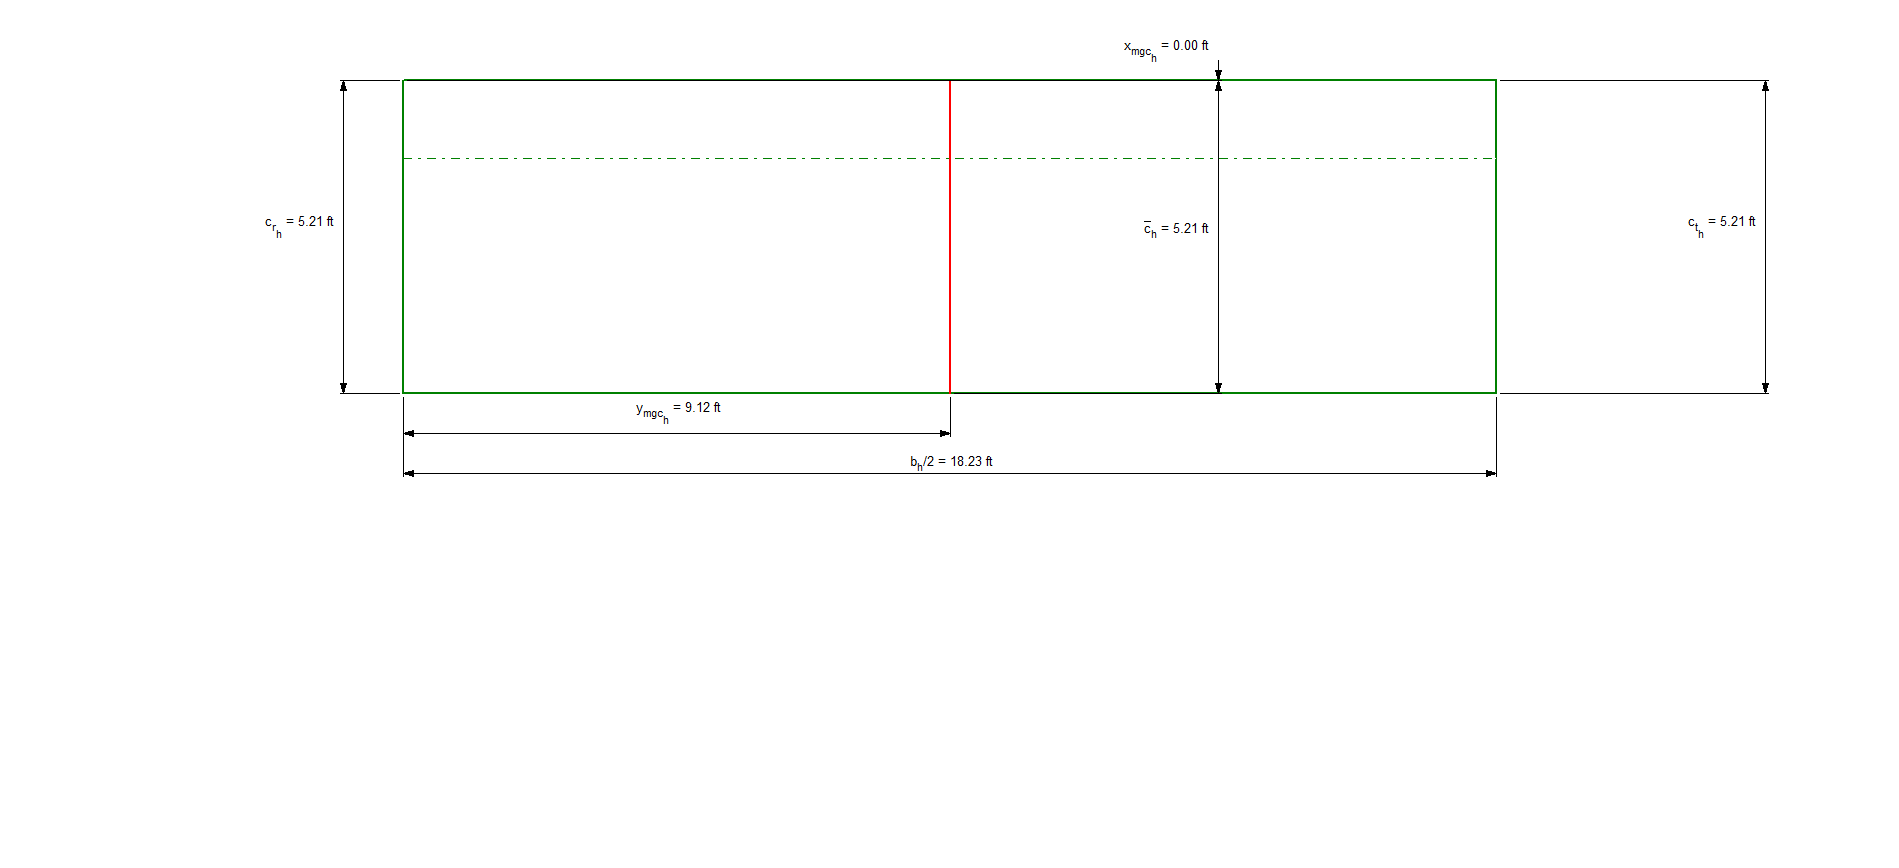
\includegraphics[width=\textwidth]{Report3Printouts/Empannage/Horizontal_geometry_plot.png}
    \caption{Horizontal stabilizer layout}
    \label{fig:horizontal_geometry_plot}
\end{figure}


\subsection{Sizing the Vertical Stabilizer}
% Discuss the location and design of the vertical stabilizer. Need to include: 
% S, b, AR, Gamma c/4, lambda, t/c, and airfoil selected. Calculate and compare 
% values of Vv to those of similar aircraft. Include AAA printouts of volume 
% coefficient calculations in the appendix and a drawing of the vertical 
% stabilizer in the chapter itself Perform a Mach critical check, if applicable. 
% Again Mcr plots are found in Canvas. Show where your point lies on the plot 
% Go to the stability and control module and calculate the static margin, 
% setting eta hp,off =1. This will give you the static margin of your airplane, 
% which is listed as the output parameter, SM. Comment on the results - is your 
% airplane likely to be longitudinally stable? Unstable? If changes need to be 
% made to either the CG (due to weight and balance) and/or the AC (due to 
% wing/tail location), now is the time to make changes.

Like the horizontal stabilizer, vertical stabilizer sizing and placement was driven primarily by the vertical tail volume ratio, $V_v$. In table 8.6b of \cite{orange_book}, all the volume ratios are between 0.065 and 0.120. A volume ratio of 0.0774 was eventually settled on, with the rest of the parameters in table \ref{tab:vertical_stabilizer_size} balanced between placement on the aircraft and control surface size. These results are from figures \ref{fig:vertical_geometry} and \ref{fig:vertical_volumeratio}. Like the horizontal stabilizer, the vertical stabilizer uses a NACA 0012 airfoil.

\begin{table}[H]
\centering
\caption{Vertical stabilizer dimensions}
\begin{tabular}{|c|c|c|c|c|c|c|c|c|c|c|}\hline
    $AR_v$ & $t/c$ & $S_v$ $[ft^2]$ & $b_v$ $[ft]$ & $\lambda_v$ & $\Lambda_{c/4_v}$ $[deg]$ & $X_{apex_v}$ $[ft]$ & $\bar{c}_v$ $[ft]$ & $c_{r_v}$ $[ft]$ & $c_{t_v}$ $[ft]$ & $V_v$ \\ \hline
    3.0 & 12\% & 137.0 & 20.27 & 0.80 & 5.0  & 60.00 & 6.79 & 7.51 & 6.01 & 0.0774 \\ \hline
\end{tabular}
\label{tab:vertical_stabilizer_size}
\end{table}

\begin{figure}[H]
    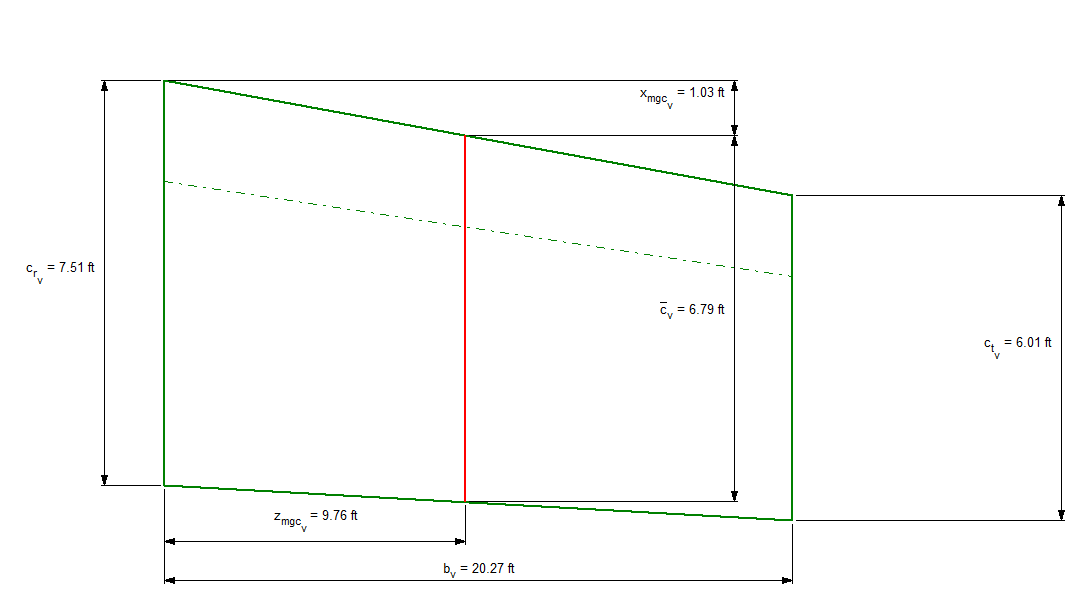
\includegraphics[width=\textwidth]{Report3Printouts/Empannage/Vertical_geometry_plot.png}
    \caption{Vertical stabilizer layout}
    \label{fig:vertical_geometry_plot}
\end{figure}


\section{Control Surface Layout Design}
\subsection{Sizing the Lateral Control Surfaces}
% Include the AAA printout of aileron calculations in the appendix and a drawing of 
% the wing/aileron in the chapter itself
% Include ca/cw, eta ai and eta ao dimensions, and show that the ailerons does not 
% interfere with the flap location. Include spoiler sizing data here if spoilers are 
% needed. Include (Sa/Sw) calculated from your AAA values and compare it with similar 
% aircraft. Comment - based on your valued, do you expect problems with sufficient roll 
% authority?

The aileron was sized to take up the remaining room on the wing, given the practical constraints that some room should be left between it and the flap for possible hinges and some space should also be left at the wingtip for navigation lights and strobes. The resulting numerical dimensions are shown in figure \ref{fig:aileron_sizing} in the Appendix and figure \ref{fig:aileron_sizing_plot} below, as well as being tabulated in table \ref{tab:aileron_size_table}. The aileron maintains a constant chord ratio ($c_a/c_w$) throughout.

\begin{table}[H]
\centering
\caption{Aileron dimensions}
\begin{tabular}{|c|c|c|c|}\hline
    $c_a/c_w$ & $\eta_{a_i}$ & $\eta_{a_o}$ & $S_a/S_w$ \\ \hline
    25.0\%    & 60.0\%     & 98.0\%     & 0.039     \\ \hline
\end{tabular}
\label{tab:aileron_size_table}
\end{table}

Given an aileron area, $S_a$ of 32.29 square feet from figure \ref{fig:aileron_sizing}, $S_a/S_w$ is calculated to be 0.039. Comparing this to other, similar aircraft is very difficult because aileron dimensions are not readily available online. Instead, three-views of three of the similar aircraft were found and the aileron span dimensions were calculated and are shown in table \ref{tab:similar_ailerons below}. For each of the aircraft where a good three-view drawing could be found, the aileron dimension calculations were performed by measuring the distance between the wingtip and aircraft centerline in pixels, as well as the distance from the centerline to the inside and outside of the aileron. $\eta_{a_i}$ would then be the distance from the centerline to the inboard side of the aileron divided by the half span.

\begin{table}[H]
\centering
\caption{Aileron spans of similar aircraft}
\begin{tabular}{|c|c|c|c|}\hline
    Aircraft & $\eta_{a_i}$ & $\eta_{a_o}$ \\ \hline
    DHC-4 & 67.0\%          & 96.0\%        \\ \hline
    DHC-6 & 44.0\%          & 95.6\%        \\ \hline
    F-27  & 70.7\%          & 98.5\%        \\ \hline
\end{tabular}
\label{tab:similar_ailerons}
\end{table}

Of these aircraft, only the DHC-6 has larger control surfaces. This makes sense because it is a bush plane which needs very good roll authority at low speed. While such large control surfaces are admirable, their necessitiy is not proven in the case of the Twin Sea Lion. The aircraft's wingspan both give the ailerons a comparitively large moment arm for roll authority and limit the number of airstrips where nimble roll control might be required.


\begin{figure}[H]
    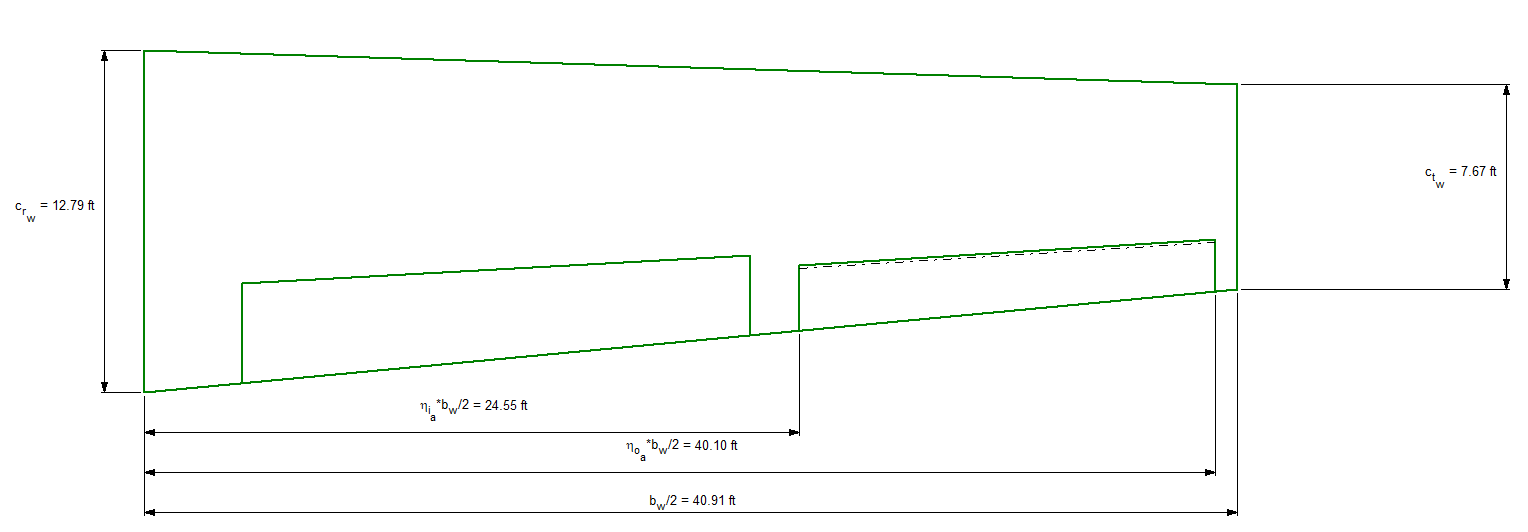
\includegraphics[width=\textwidth]{Report3Printouts/Wing_and_Aileron/aileron_sizing_plot.png}
    \caption{Aileron layout on the Twin Sea Lion}
    \label{fig:aileron_sizing_plot}
\end{figure}

\subsection{Sizing the Longitudinal Control Surfaces}
% Include AAA printout of elevator and/or canardvator calculations in the appendix 
% and a drawing of the tail/elevator and/or canard/canardvator in the chapter itself
% Include ce/ch, eta eo dimensions (and/or ccv/cc, eta cvi, and eta cvo dimensions). 
% Include (Se/Sh), and/or (Scv/Sc) calcuated from your AAA values and compare them with 
% similar aircraft. Comment - based on your values, do you expect problems with 
% sufficient pitch authority?
% If you have a movable stabilizer with no elevator and/or a movable canard with no 
% canardvator, state and discuss that in this section

As seen in figure \ref{fig:horizontal_elevator}, Elevator design was kept as simple as possible. $C_e/C_h$ was kept at 30\% for the entire length of the elevator, which runs from 5\% to 95\% of the horizontal stabilizer half span. The elevator area, $S_e$, is 48.74 square feet of the 190 square feet of the entire horizontal stabilizer, $S_h$.

\begin{table}[H]
\centering
\caption{Elevator dimensions}
\begin{tabular}{|c|c|c|c|}\hline
    $c_e/c_h$ & $\eta_{e_i}$ & $\eta_{e_o}$ & $S_e/S_h$ \\ \hline
    30.0\%    & 5\%          & 95.0\%       & 0.256     \\ \hline
\end{tabular}
\label{tab:elevator_size_table}
\end{table}

Based on the substantial control surfaces, a properly balanced aircraft would 
be easily controllable with this tail configuration. Because the Twin Sea Lion has 
such a large static margin, this elevator may still be undersized. In either case, 
the area ratios and chord ratios of the elevator and horizontal stabilizer are in 
the range of values noted in \cite{orange_book}, which range between 0.28 and 1 for $S_e/S_h$ and 0.29 to 0.50 for $c_e/c_h$.

\begin{figure}[H]
    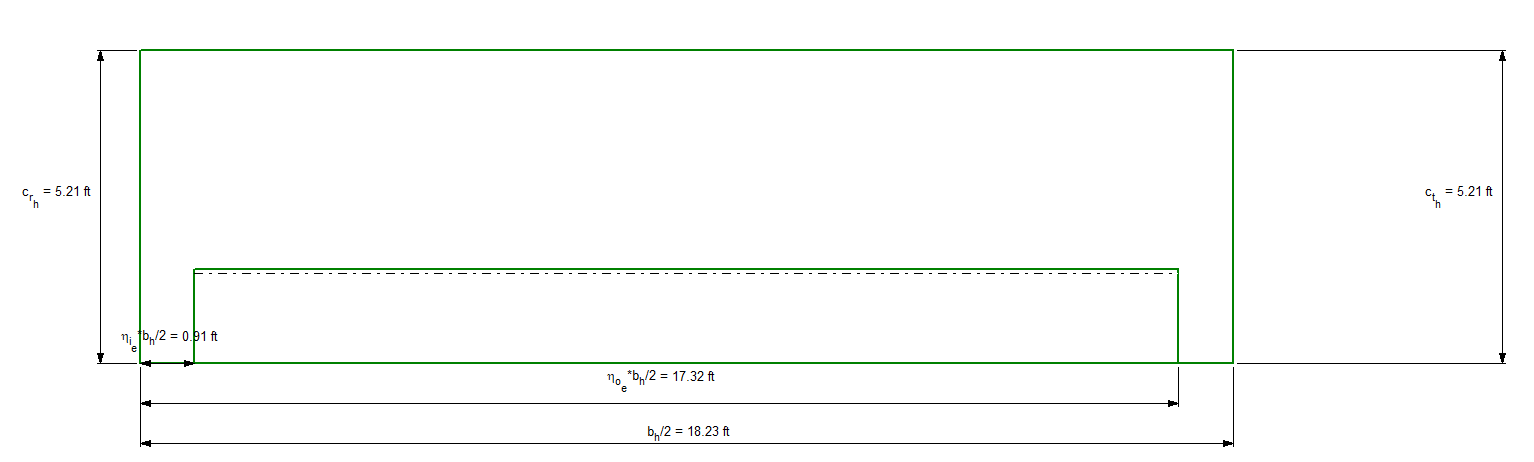
\includegraphics[width=\textwidth]{Report3Printouts/Empannage/Horizontal_elevator_plot.png}
    \caption{Elevator layout on the Twin Sea Lion}
    \label{fig:horizontal_elevator_plot}
\end{figure}

\subsection{Sizing the Directional Control Surfaces}
% Include AAA printout of rudder calculations in the appendix and a drawing of 
% the tail/rudder in the chapter itself. Include cr/cv, eta ri and eta r0 dimensions. 
% Include (Sr/Sv) calculated from your AAA values and compare it with similar aircraft. 
% Comment - based on your values, do you expect problems with sufficient yaw authority?

The rudder was sized according to figure \ref{fig:vertical_rudder}. Its dimensions are very similar to those of the elevators. The geometry is summarized in table \ref{tab:rudder_size_table} below. The total rudder area, $S_r$, is 35.14 square feet, making $S_r/S_v = 0.256$. Looking at \cite{orange_book} again, most reigonal turboprop aircraft have rudders between 0.26 and 0.41 of the total vertical surface area. This means that some issues with rudder authority might appear. This could be a limiting factor on the crosswind capabilities and spin recovery of the Twin Sea Lion.

\begin{table}[H]
\centering
\caption{Rudder dimensions}
\begin{tabular}{|c|c|c|c|}\hline
    $c_r/c_v$ & $\eta_{r_i}$ & $\eta_{r_o}$ & $S_r/S_v$ \\ \hline
    30.0\%    & 5\%          & 95.0\%       & 0.256     \\ \hline
\end{tabular}
\label{tab:rudder_size_table}
\end{table}

\begin{figure}[H]
    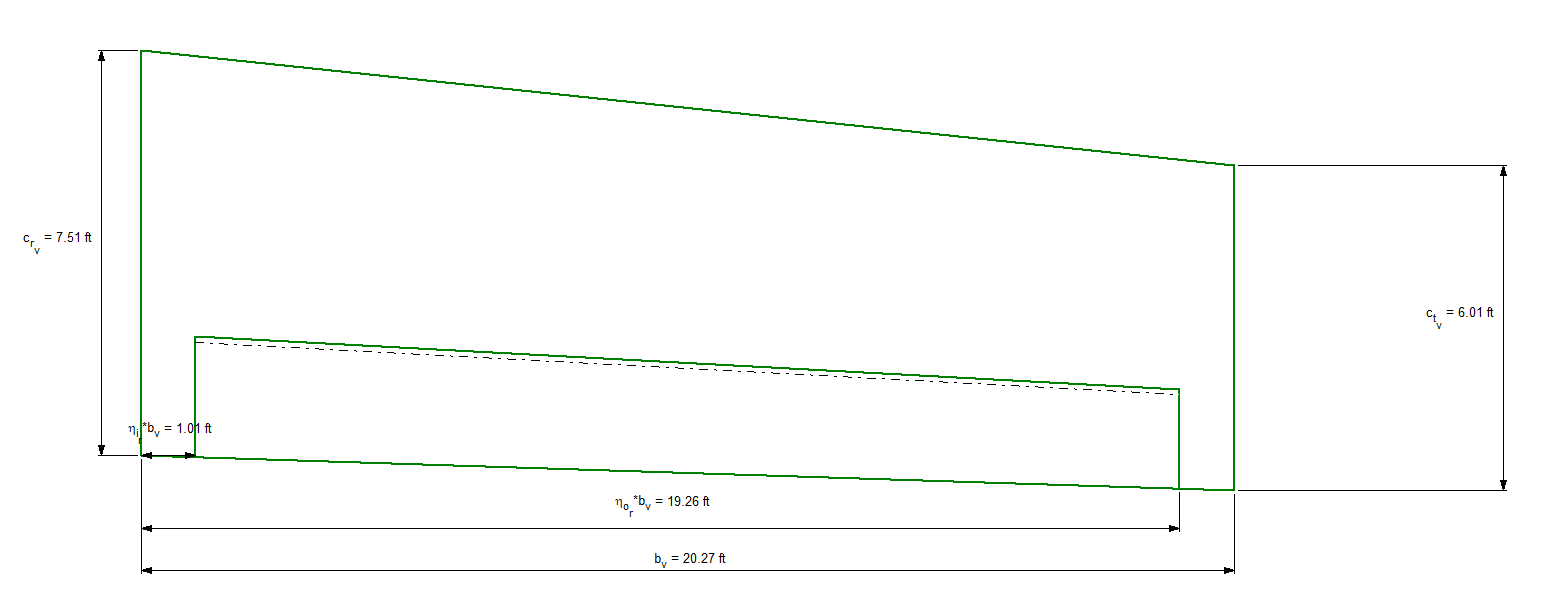
\includegraphics[width=\textwidth]{Report3Printouts/Empannage/Vertical_rudder_plot.png}
    \caption{Rudder control surface layout}
    \label{fig:vertical_rudder_plot}
\end{figure}



%\section{Landing Gear Layout Design}
%\subsection{Sizing of the Landing Gear}
%Describe how you chose the landing gear configuration (tricycle, taildragger, etc) for your aircraft and why.
% Include
	%Fixed or retractable
    %Number of struts ("bogeys")
    %Number of tires per strut and selection of tires (diameter and width)
    %Arrangement of tires (dual, tandem, etc)
    %Maximum static load per bogey (Pn and Pm)
    %Weight distribution % - is it within acceptable bounds?
%\subsection{Location of the Landing Gear}
%Describe how you chose the location of the gear for your aircraft
%Show that you meet longitudinal and lateral ground clearance requirements
%Show that you meet longitudinal and lateral tip-over requirements
%Include strut diameters and lengths


%\subsection{Gear Retraction Volume}
%If application, discuss your gear retraction volume calculations (with growth factors) for all gear and whether the gear will retract into the wings, into the fuselage, or a bubble fairing on the side of the fuselage. Show your calculations, both for what volume is required for retraction and for what is available in the wing, fuselage, or fairing.

\section{Conclusions and Recommendations}
\subsection{Conclusions}

\subsection{Recommendations}

\begin{thebibliography}{99}

% Todo: orange book charts for Vh and Vv

\bibitem{pres18} Gerren, "Presentation 18", \url{https://canvas.colorado.edu}

\bibitem{pres19} Gerren, "Presentation 19", \url{https://canvas.colorado.edu}

\bibitem{orange_book} Roskam, "Tail and Control Surface Info", \url{https://canvas.colorado.edu}

\bibitem{gear info} Roskam, "Landing Gear Sizing", \url{https://canvas.colorado.edu}

\bibitem{roskam 3} Roskam, "Center of Gravity Ranges", Table 10.3, \url{https://canvas.colorado.edu}

\bibitem{aircraft dynamics} Etkin and Reid, \textit{Dynamics of Flight} "Stability and Control, Third Edition." 1996,John Wiley \& Sons, Inc.

% Twin Otter: https://www.vikingair.com/sites/default/files/documents/Twin%20Otter%20Series%204
%00%20Multi-Page%20Brochure.pdf
%\bibitem{dhc-6} Twin Otter Series 400. Viking Air, 
%    \url{https://www.vikingair.com/sites/default/files/documents/Twin Otter Series 400 Multi-Pa
%ge Brochure.pdf}

% PC-24: https://www.pilatus-aircraft.com/en/fly/pc-24 | Weight from Wikipedia
% https://www.pilatus-aircraft.com/data/document/Pilatus-Aircraft-Ltd-PC-24-Factsheet.pdf
%\bibitem{pc24Wto} PC-24 The Super Versatile Jet. Pilatus, 
%        \url{http://www.pilatus-aircraft.com/data/document/Pilatus-Aircraft-Ltd-PC-24-Factsheet
%.pdf}
%empty weight: https://www.militaryfactory.com/aircraft/detail.asp?aircraft_id=1256#specs
%\bibitem{pc24We} "Pilatus PC-24 Light Passenger Jet Aircraft - Switzerland." Military Weapons, 
%    \url{http://www.militaryfactory.com/aircraft/detail.asp?aircraft_id=1256#specs}

% DHC-4: http://www.dhc4and5.org/caribou_manuals.htm
%\bibitem{dhc-4} "C-7A Flight Manual Performance Data." Wayne E. Buser, 
%    \url{http://www.dhc4and5.org/caribou_manuals.htm}

% F-27: https://www.planeandpilotmag.com/article/fairchild-hiller-fh-227-fokker/
%\bibitem{F-27} "FAIRCHILD HILLER FH-227 (FOKKER)" Plane and Pilot Magazine, 
%    \url{https://www.planeandpilotmag.com/article/fairchild-hiller-fh-227-fokker/}

% Q-400: https://www.airliners.net/aircraft-data/de-havilland-canada-dhc-8-400-dash-8/122
%\bibitem{Q400} "De Havilland Canada DHC-8-400 Dash 8." Airliners.net, 
%    \url{http://www.airliners.net/aircraft-data/de-havilland-canada-dhc-8-400-dash-8/122}

% http://www.flugzeuginfo.net/acdata_php/acdata_f27_en.php
%\bibitem{F-27-length} "Fokker F27 Friendship" Flugzeuginfo Info,
%    \url{http://www.flugzeuginfo.net/acdata_php/acdata_f27_en.php}

% Three Views
%\bibitem{dh4_threeview} "DHC-4 Three View"
%    \url{http://www.wallaby03.com/wp-content/uploads/2009/12/DHC-4A-specs.jpg}
%\bibitem{dh6_threeview} "DHC-6 Three View"
 %   \url{http://aviadejavu.ru/Images6/AN/AN82-11/27-3.jpg}
%\bibitem{f27_threeview} "F-27 Three View"
 %   \url{https://www.the-blueprints.com/blueprints-depot-restricted/modernplanes/fairchild/fairchild_f_27a-53997.jpg}

\end{thebibliography}

% 8
\section{Appendix}

\subsection{AAA: Preliminary Weight Analysis}
\begin{figure}[H]
    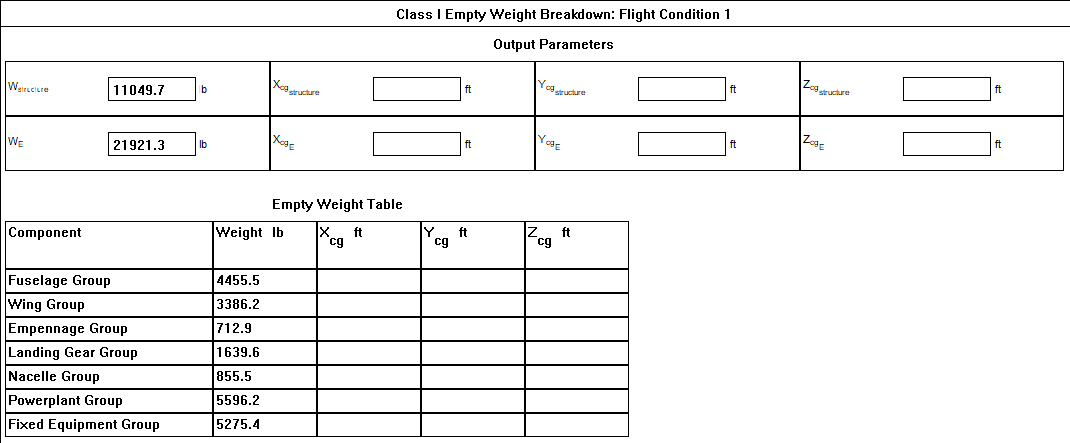
\includegraphics[width=\textwidth]{Report3Printouts/Weight/ComponentWeights_cropped.png}
    \caption{Structural component weight breakdown}
    \label{fig:componentweights}
\end{figure}

\begin{figure}[H]
    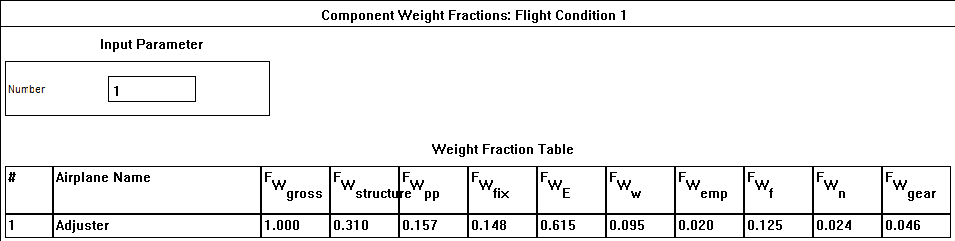
\includegraphics[width=\textwidth]{Report3Printouts/Weight/CustomAirplane_cropped.png}
    \caption{A custom airplane model used for weight allocation in AAA}
    \label{fig:customairplane}
\end{figure}

\begin{figure}[H]
    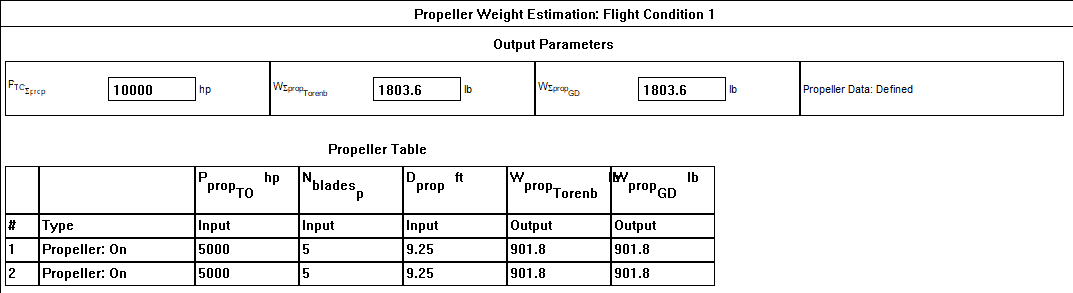
\includegraphics[width=\textwidth]{Report3Printouts/Weight/PropellerWeight_cropped.png}
    \caption{Propeller weights estimates}
    \label{fig:propellerweight}
\end{figure}

\begin{figure}[H]
    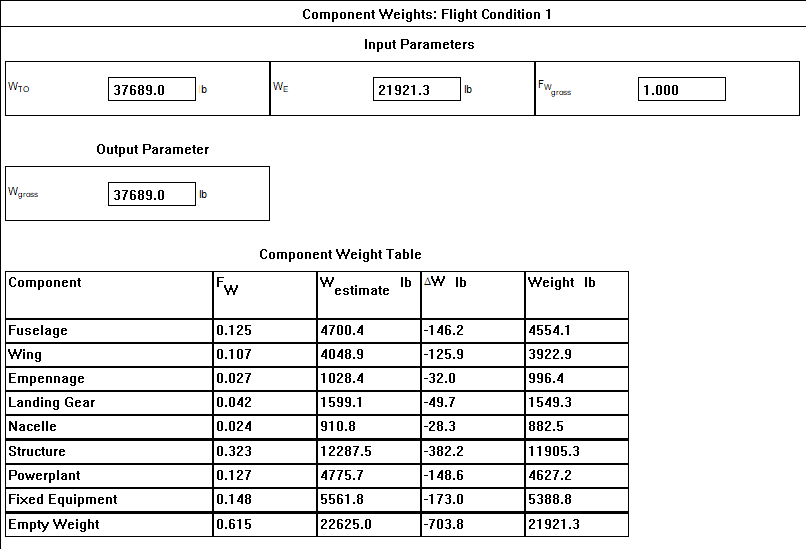
\includegraphics[width=\textwidth]{Report3Printouts/Weight/WeightFractionsInitial_cropped.png}
    \caption{Initial structural weight fractions}
    \label{fig:weightfractionsinitial}
\end{figure}

\begin{figure}[H]
    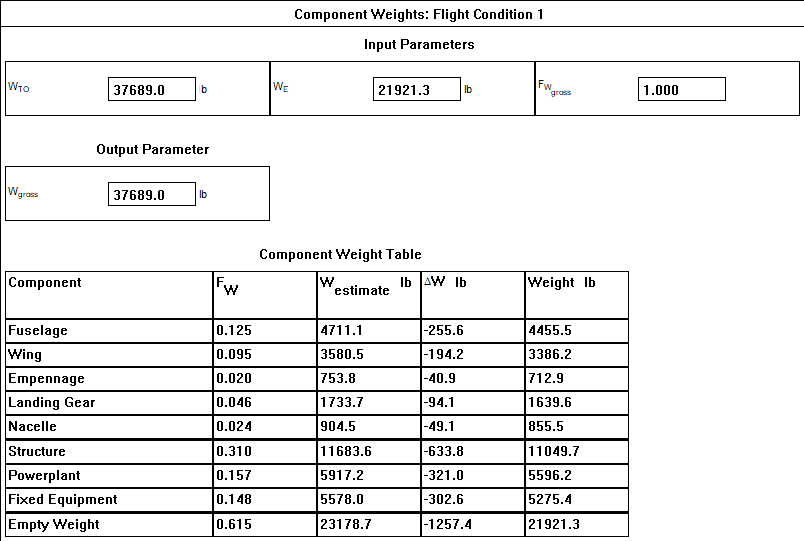
\includegraphics[width=\textwidth]{Report3Printouts/Weight/WeightFractionsFinal_cropped.png}
    \caption{Finalized structural weight fractions}
    \label{fig:weightfractionsfinal}
\end{figure}

\subsection{AAA: Preliminary Balance Analysis}

\begin{figure}[H]
    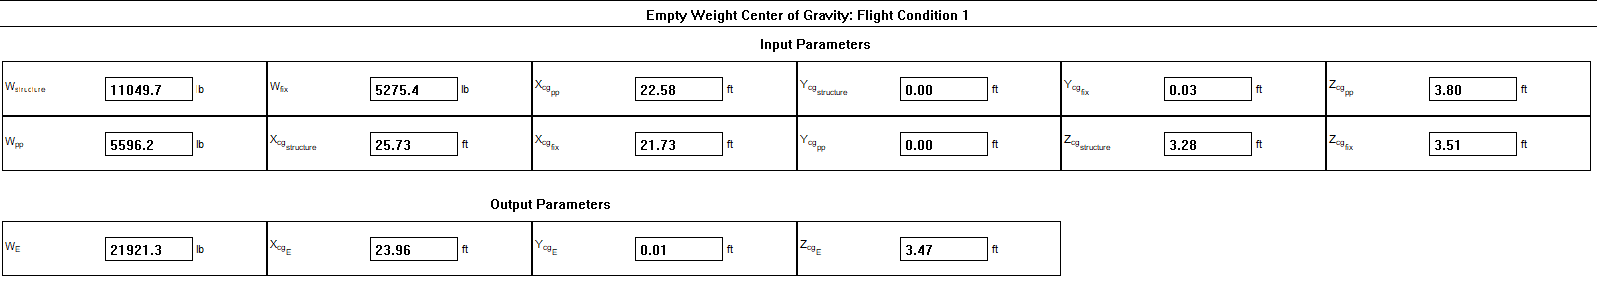
\includegraphics[width=\textwidth]{Report3Printouts/Cg/Cg_Empty_Detailed_Empty_cropped.png}
    \caption{Detailed breakdown of CG components of the empty aircraft}
    \label{fig:cg_detailed_empty}
\end{figure}

\begin{figure}[H]
    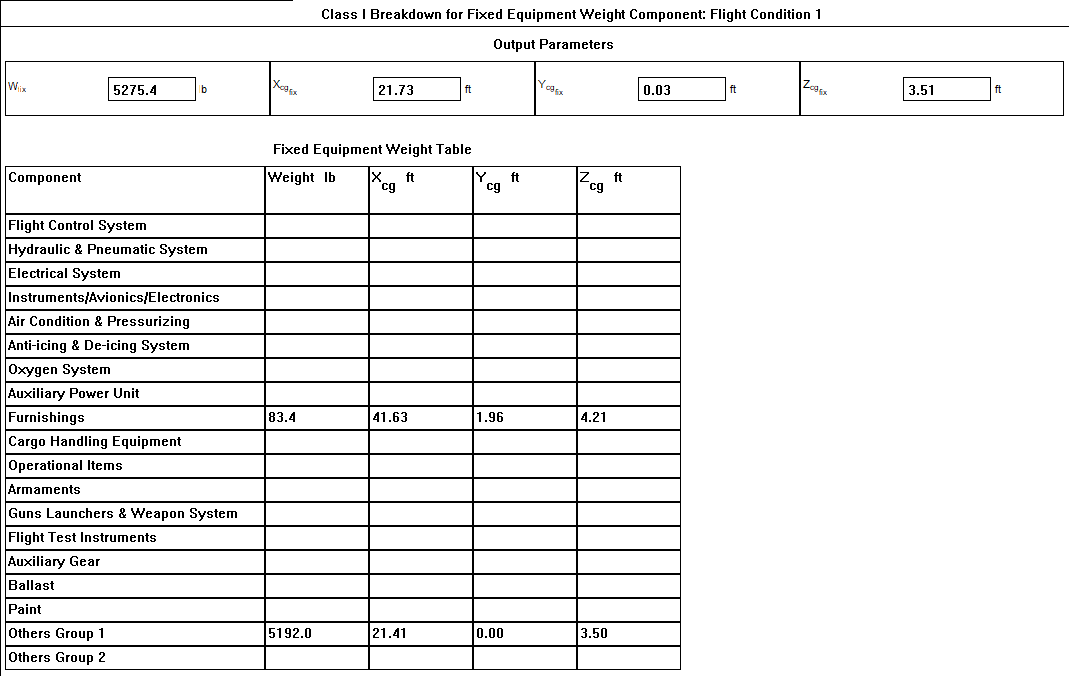
\includegraphics[width=\textwidth]{Report3Printouts/Cg/Cg_Empty_Detailed_FixedEquipment_cropped.png}
    \caption{Detailed breakdown of CG and weight of the fixed equipment}
    \label{fig:cg_empty_detailed_fixedequipment}
\end{figure}

\begin{figure}[H]
    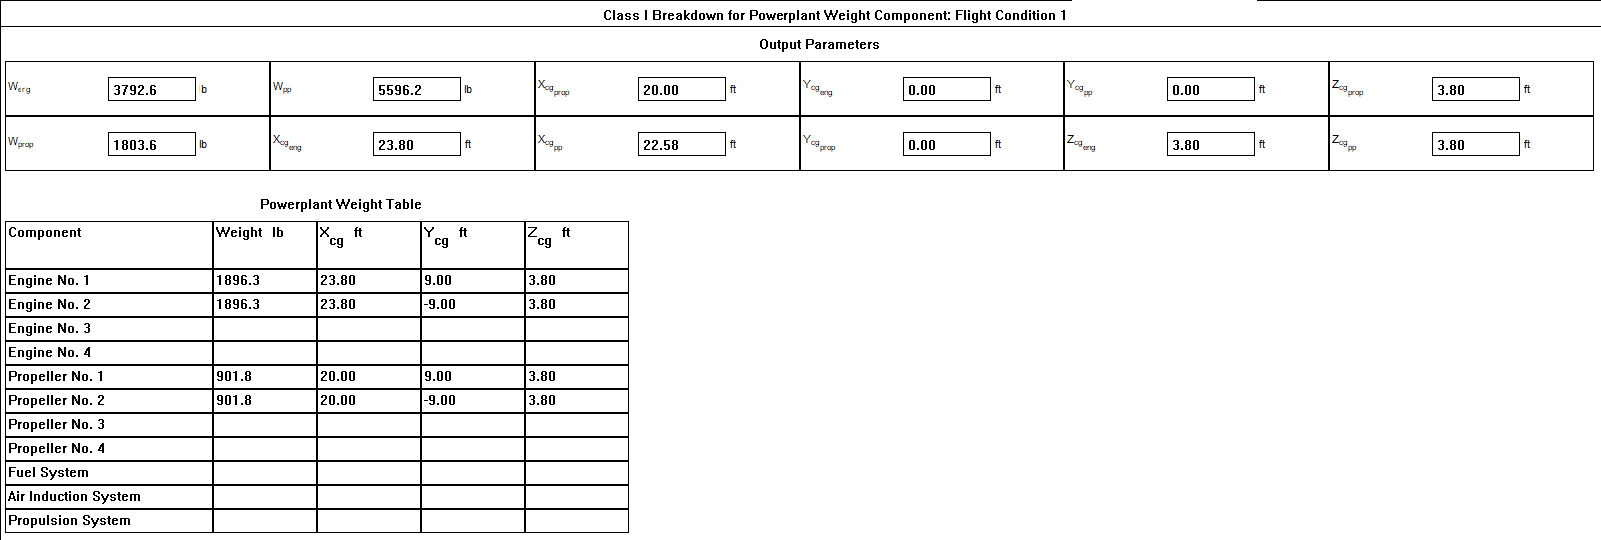
\includegraphics[width=\textwidth]{Report3Printouts/Cg/Cg_Empty_Detailed_Powerplant_cropped.png}
    \caption{Powerplant CG breakdown}
    \label{fig:cg_empty_detailed_powerplant}
\end{figure}


\begin{figure}[H]
    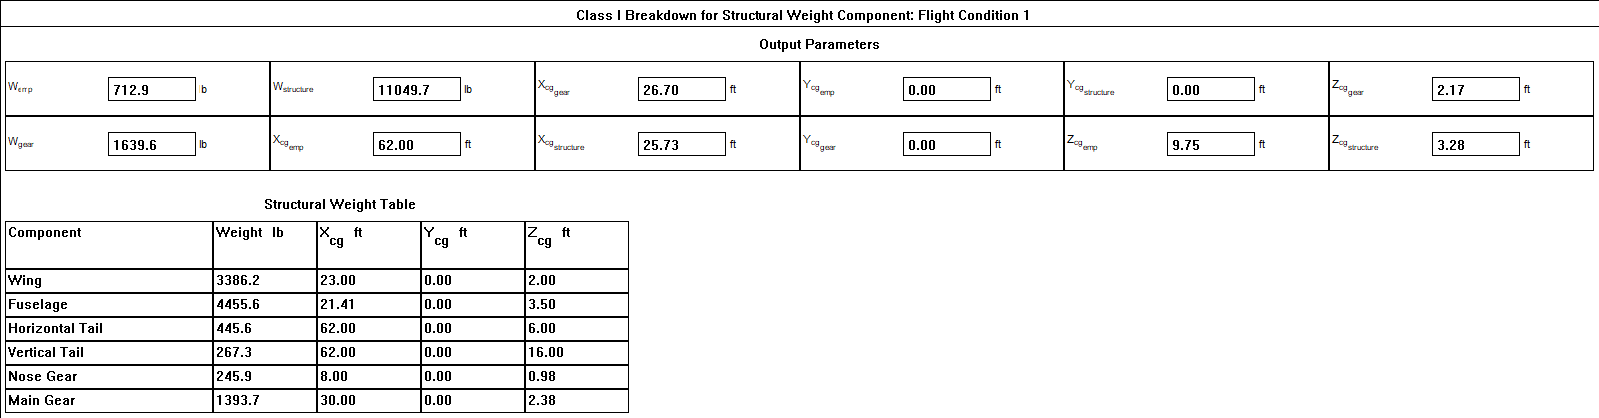
\includegraphics[width=\textwidth]{Report3Printouts/Cg/Cg_Empty_Detailed_Structure_cropped.png}
    \caption{Structure CG breakdown}
    \label{fig:cg_empty_detailed_structure}
\end{figure}


\begin{figure}[H]
    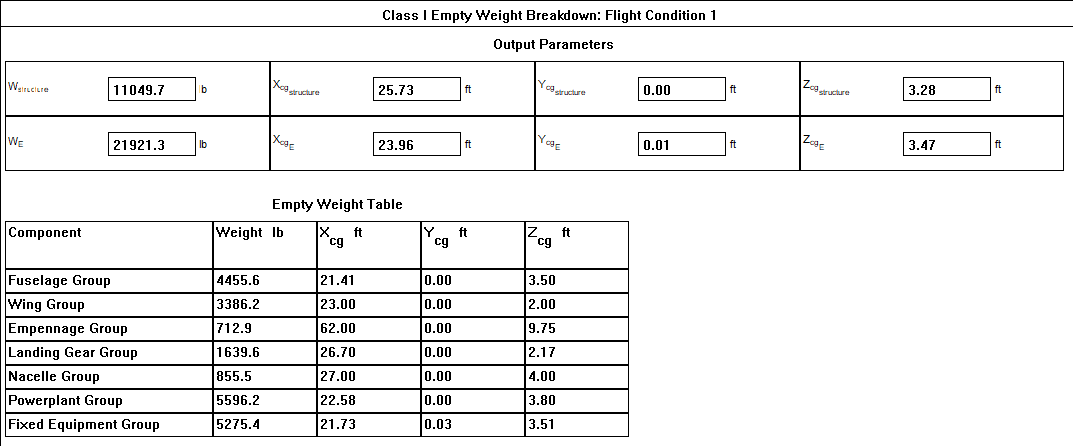
\includegraphics[width=\textwidth]{Report3Printouts/Cg/Cg_Empty_Fractions_cropped.png}
    \caption{Equipment group CG breakdown}
    \label{fig:cg_empty_fractions}
\end{figure}


\begin{figure}[H]
    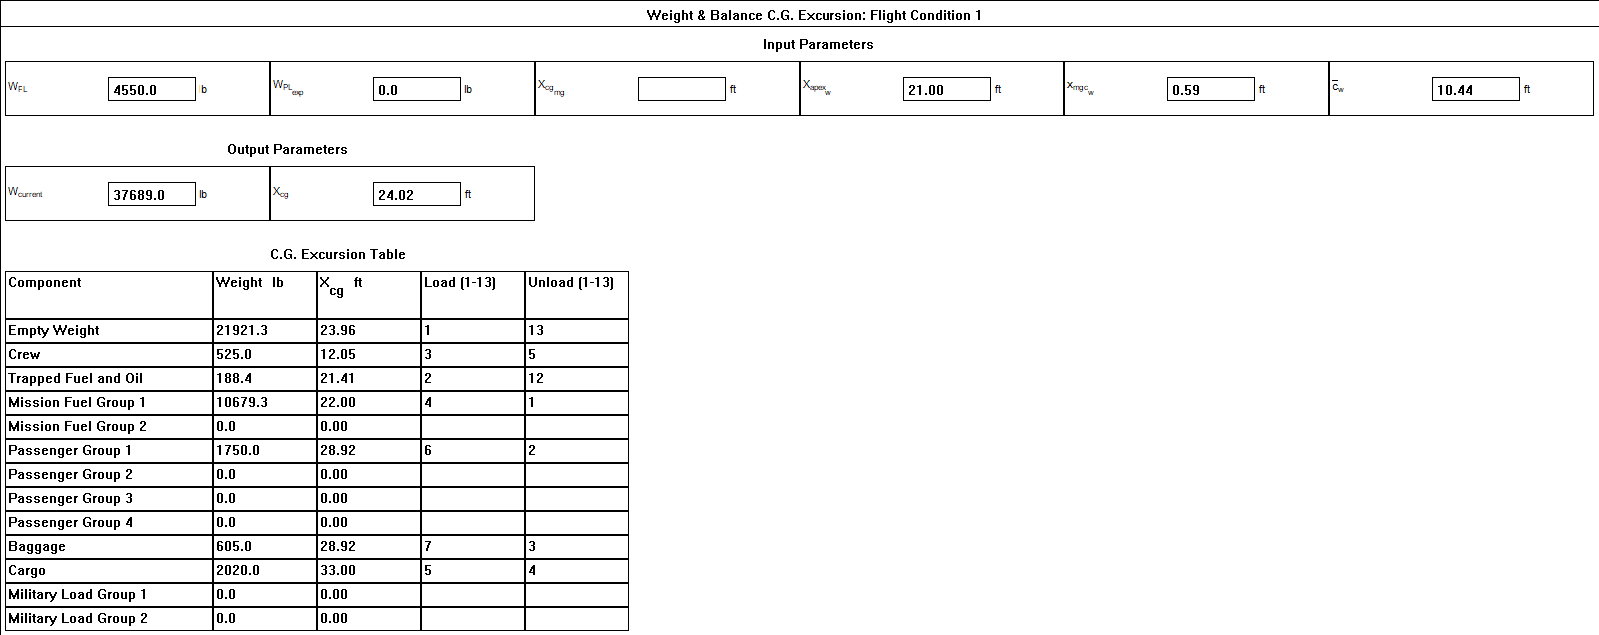
\includegraphics[width=\textwidth]{Report3Printouts/Cg/Cg_Excursion_cropped.png}
    \caption{CG excursion ordering}
    \label{fig:cg_excursion}
\end{figure}

\begin{figure}[H]
    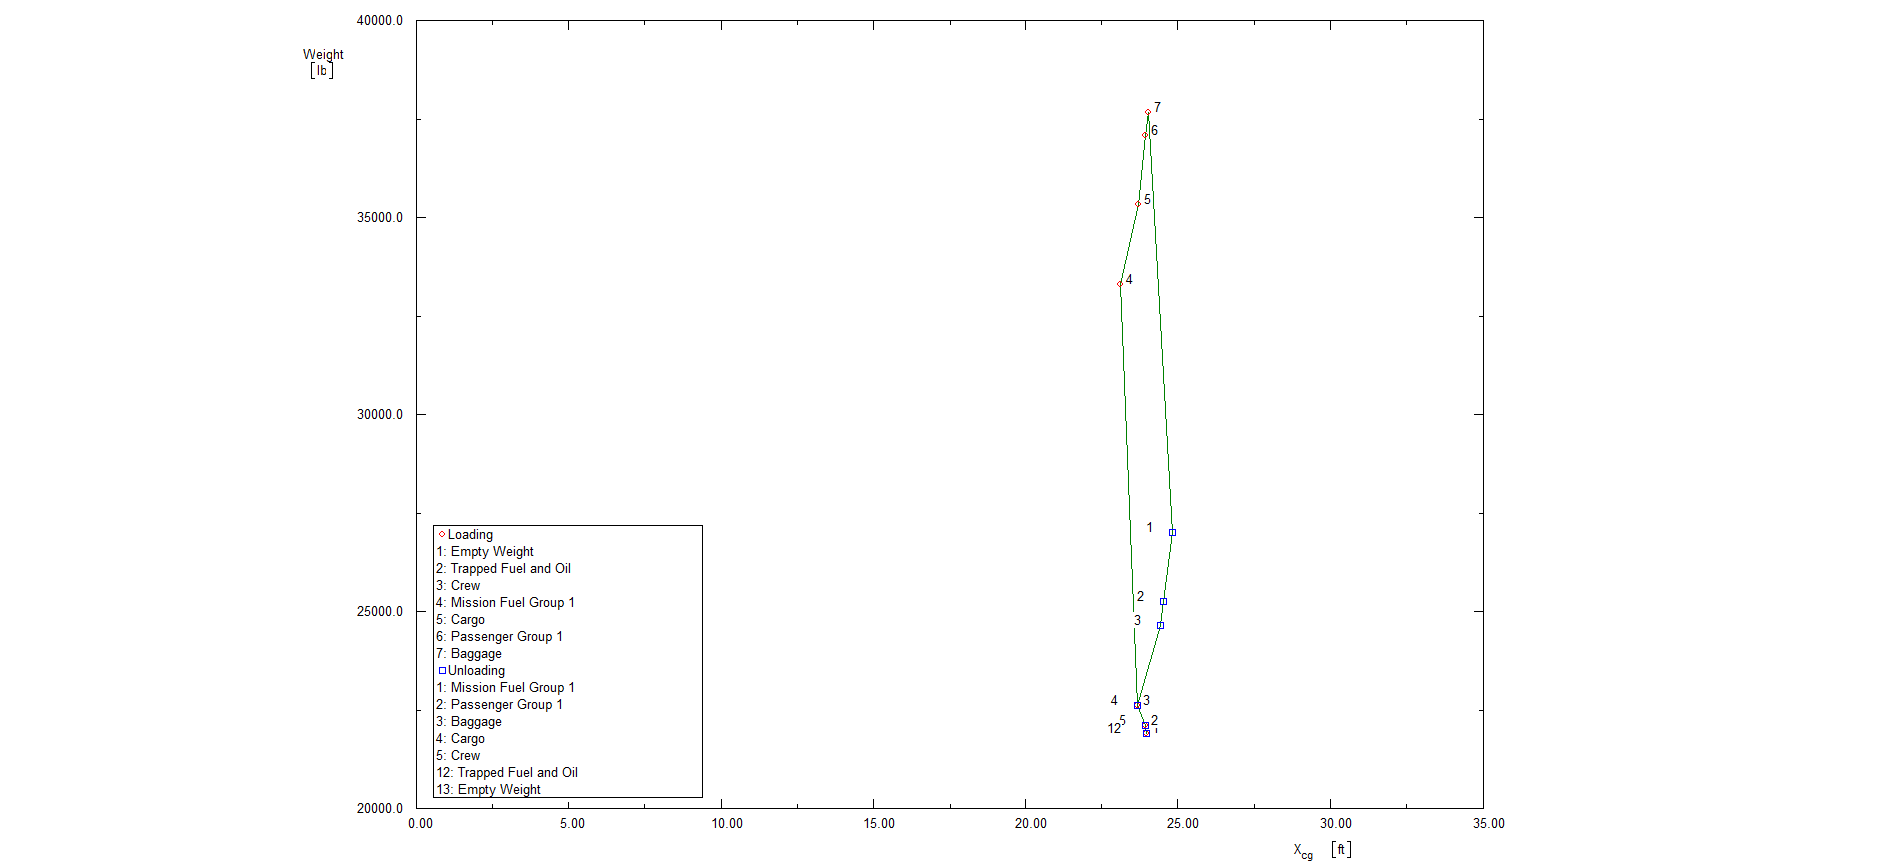
\includegraphics[width=\textwidth]{Report3Printouts/Cg/Cg_Excursion_Plot_cropped.png}
    \caption{Plot of CG excursion}
    \label{fig:cg_excursion_plot}
\end{figure}

\begin{figure}[H]
    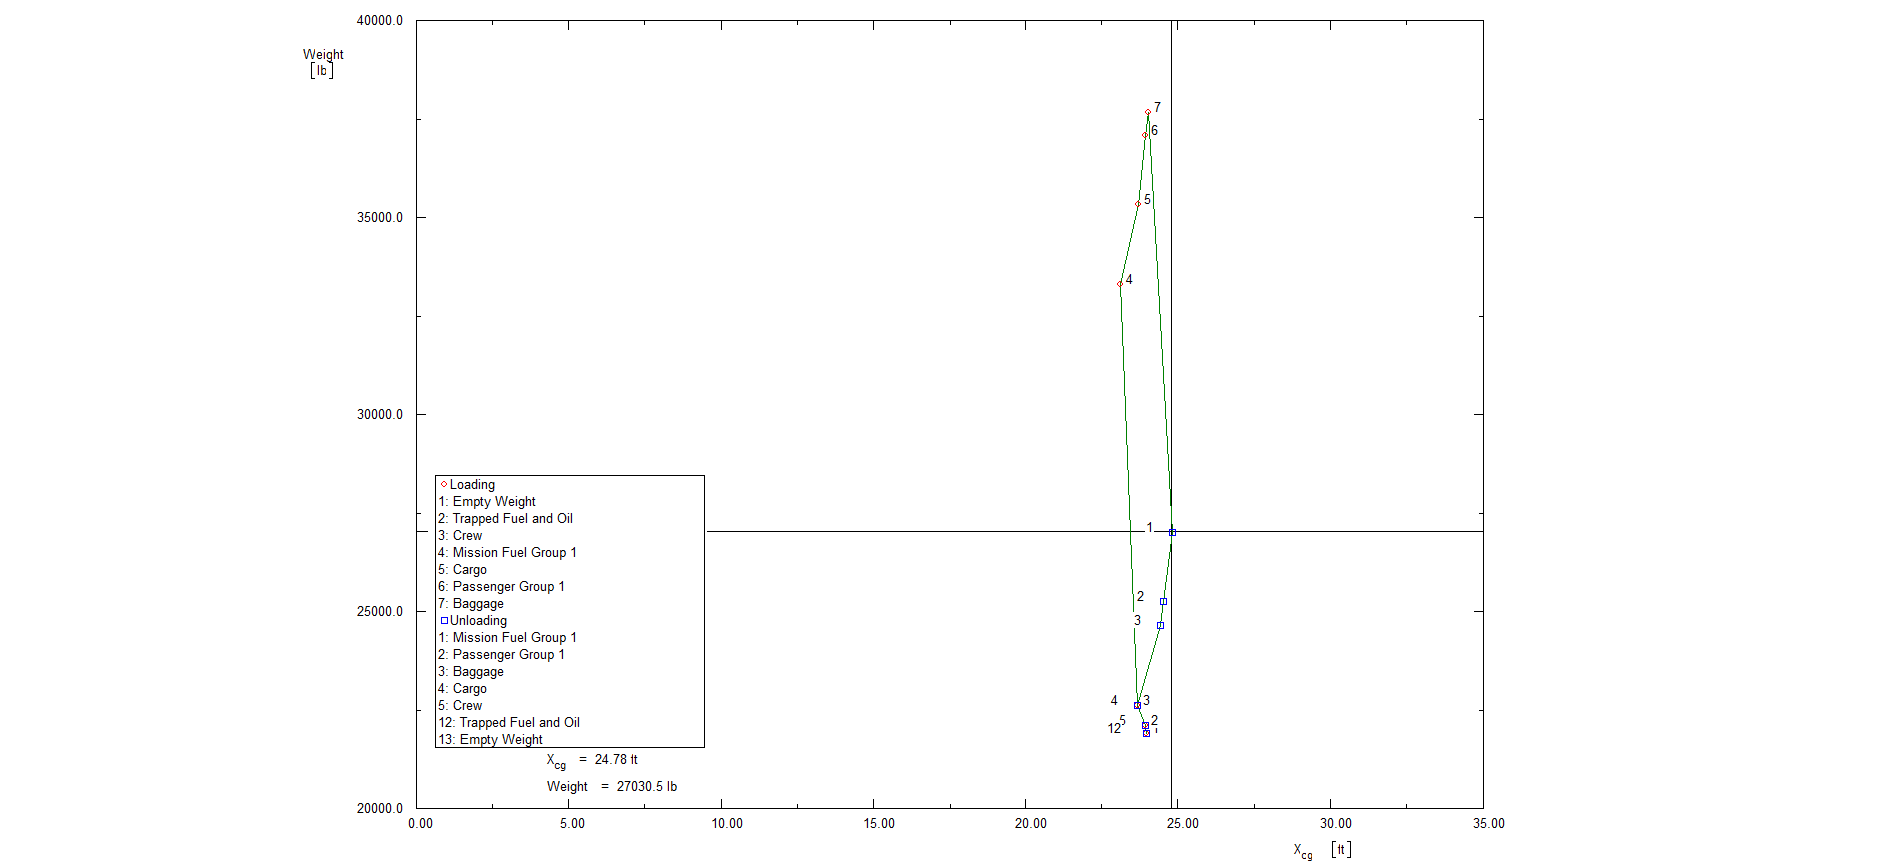
\includegraphics[width=\textwidth]{Report3Printouts/Cg/Cg_excursion_plot_mostaft_cropped.png}
    \caption{Plot of CG excursion with most aft point marked}
    \label{fig:cg_excursion_plot_mostaft}
\end{figure}


\begin{figure}[H]
    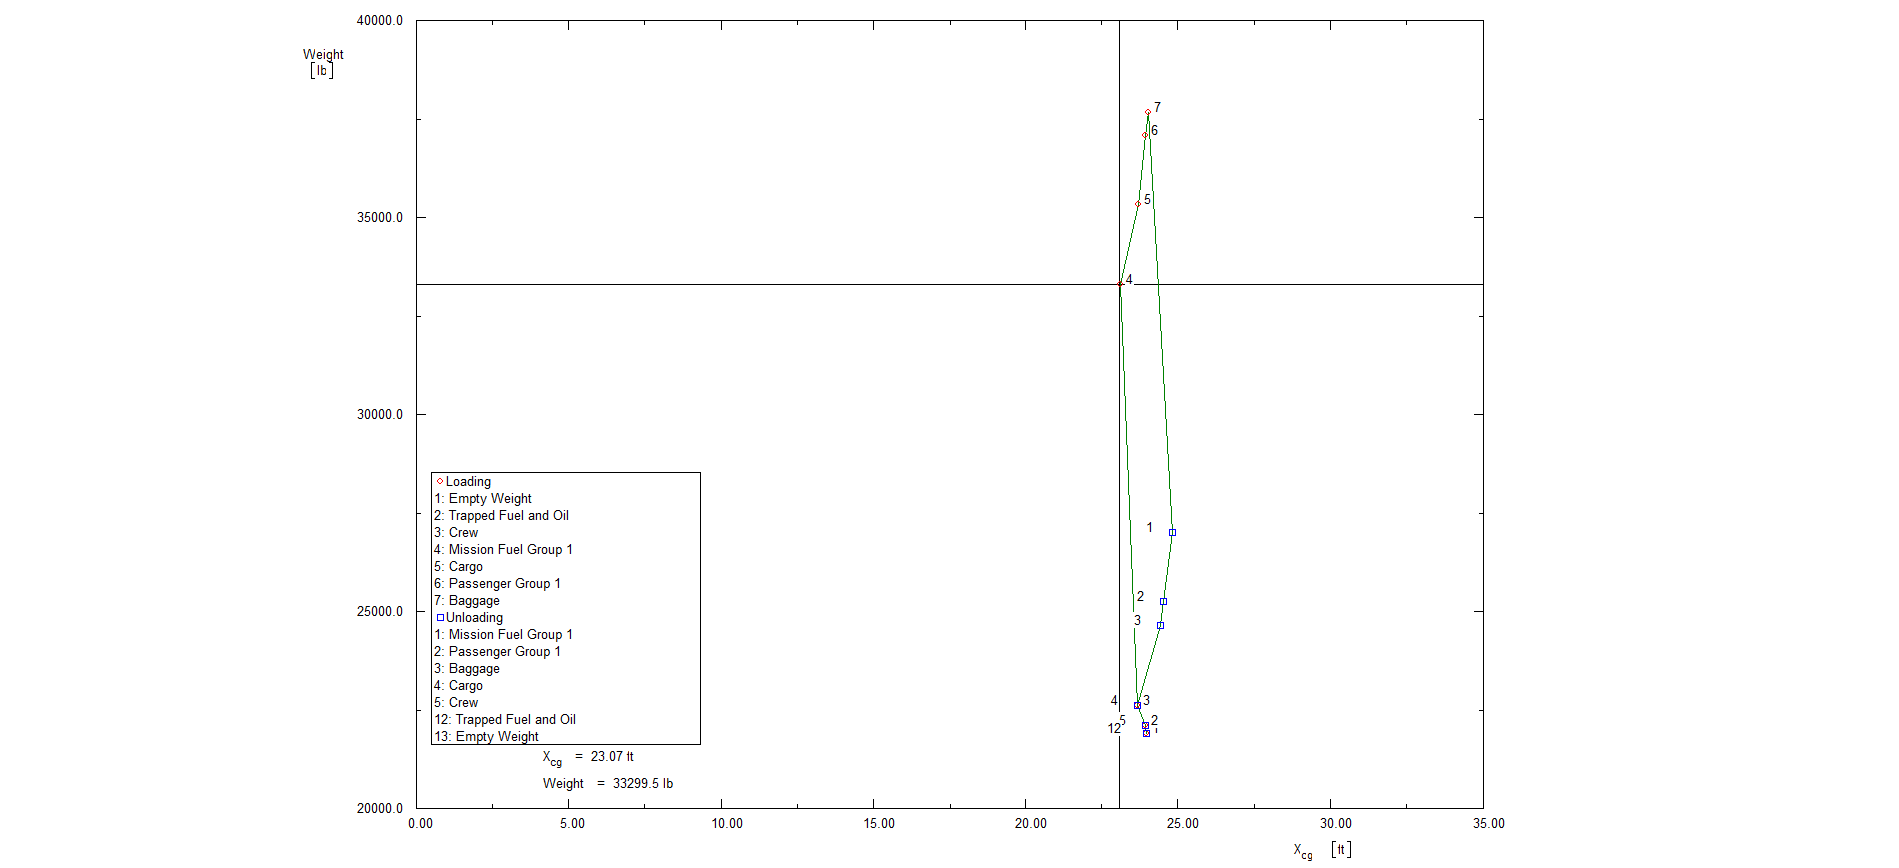
\includegraphics[width=\textwidth]{Report3Printouts/Cg/Cg_excursion_plot_mostforward_cropped.png}
    \caption{Plot of CG excursion with most forward point marked}
    \label{fig:cg_excursion_plot_mosforward}
\end{figure}

\begin{figure}[H]
    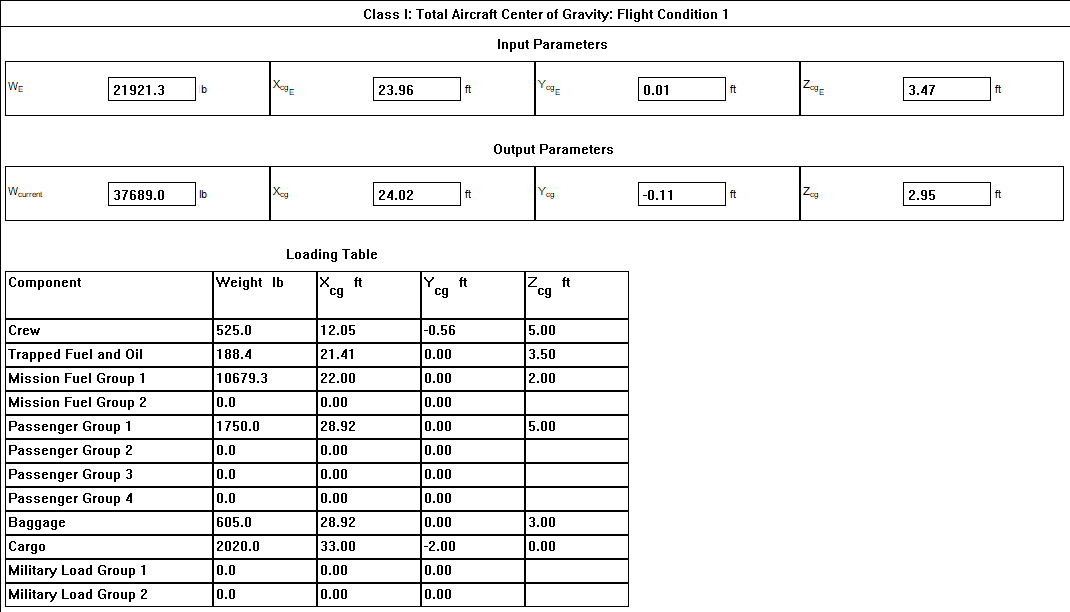
\includegraphics[width=\textwidth]{Report3Printouts/Cg/Cg_TotalAircraft_cropped.png}
    \caption{Fully loaded aircraft CG breakdown}
    \label{fig:cg_totalaircraft}
\end{figure}

\subsection{AAA: Empennage Layout Design}

\begin{figure}[H]
    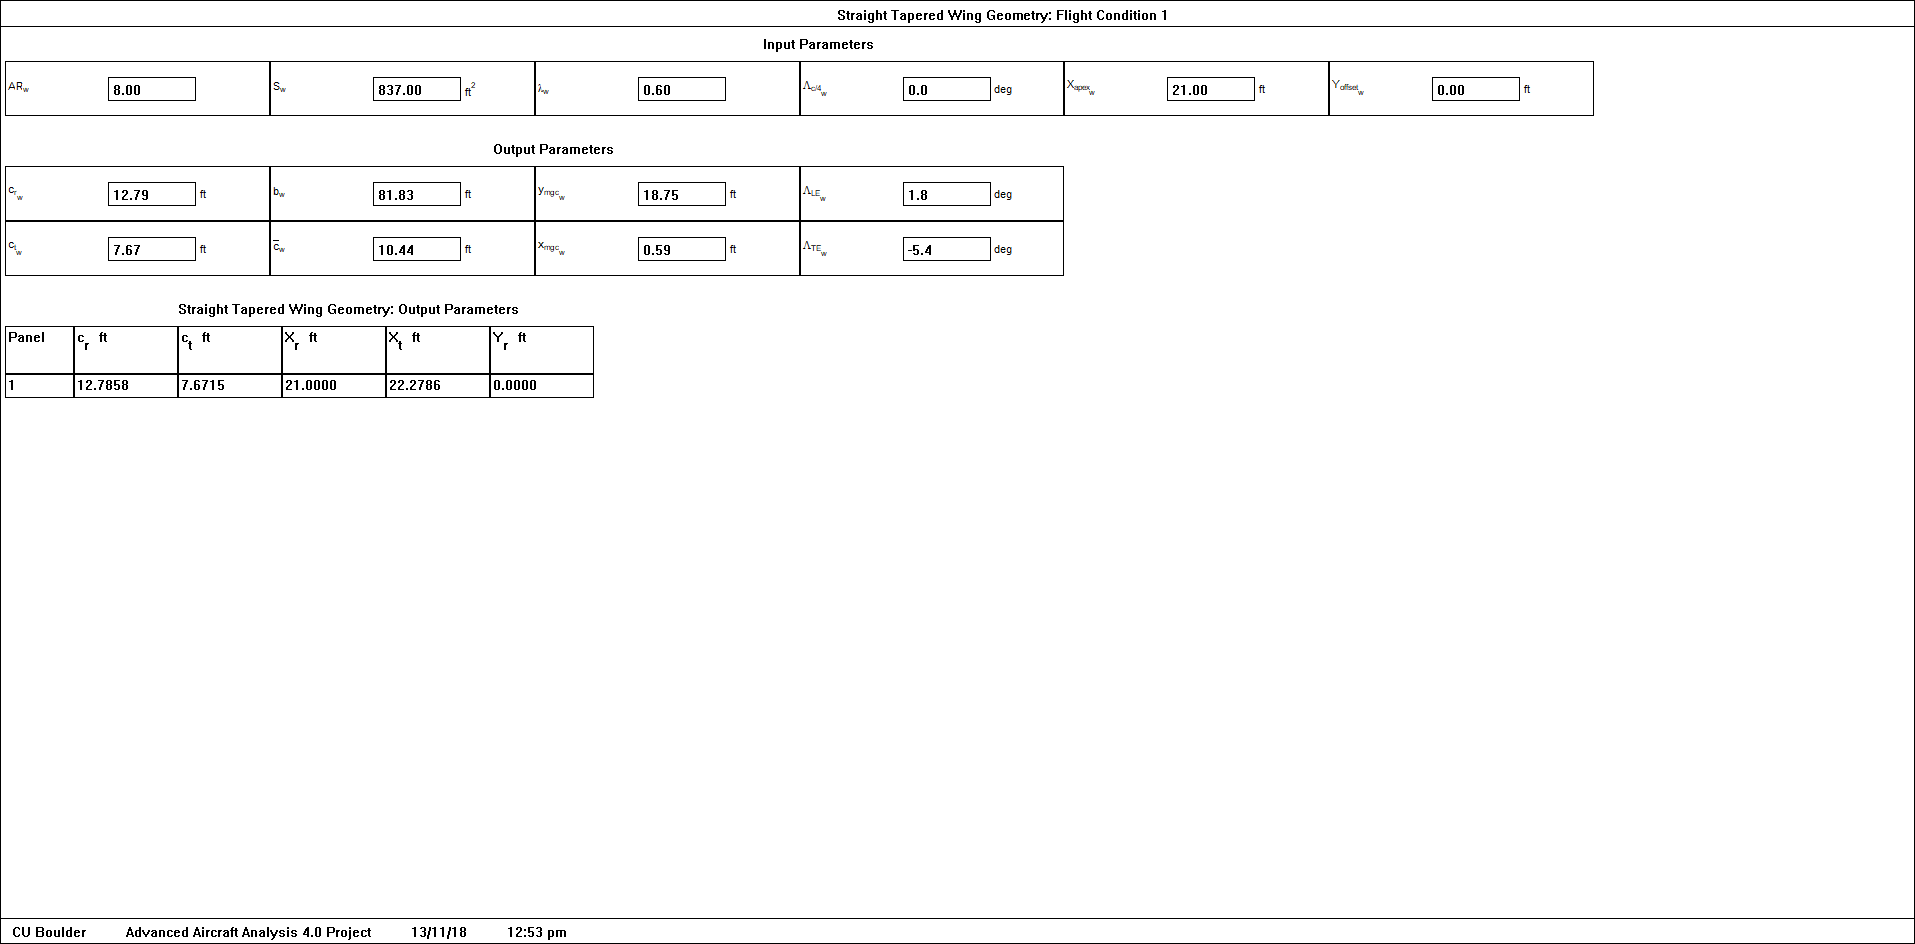
\includegraphics[width=\textwidth]{Report3Printouts/changedwing.png}
    \caption{Wing layout, with adjusted apex location}
    \label{fig:changedwing}
\end{figure}

\begin{figure}[H]
    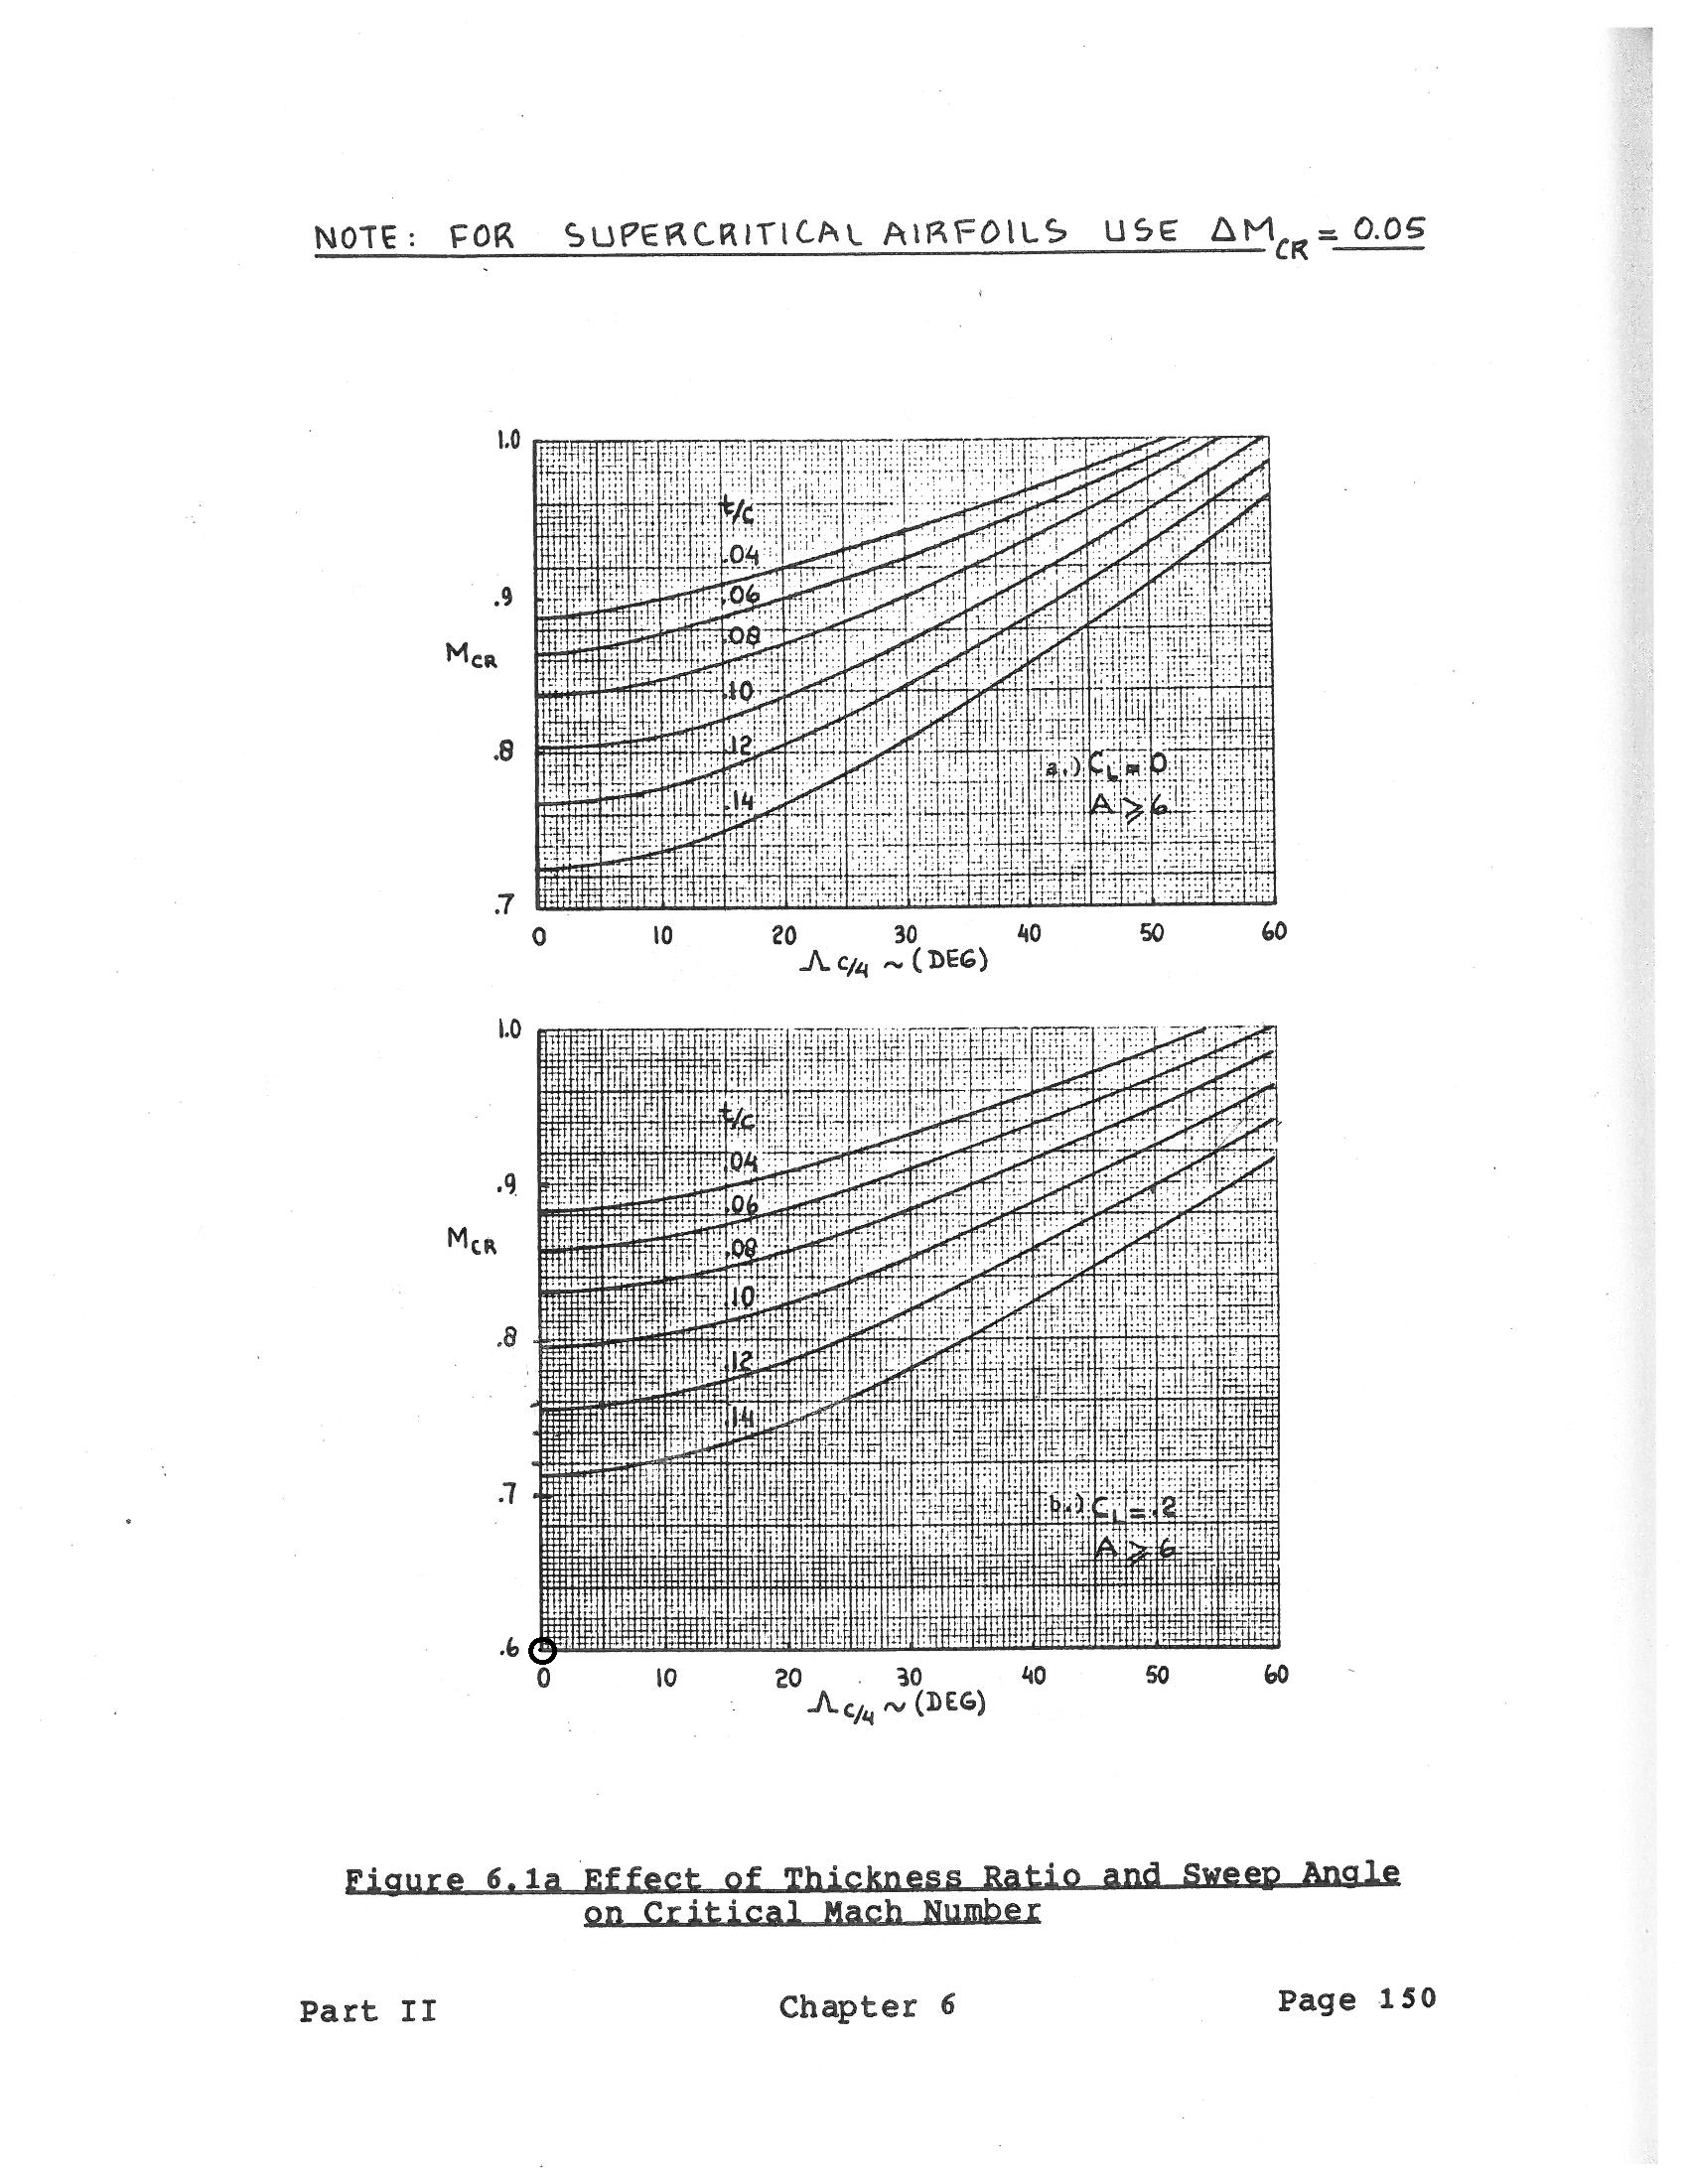
\includegraphics[width=\textwidth]{plots/Mcr_check.png}
    \caption{Critical Mach number checks for shockwave formation on an airfoil}
    \label{fig:critical_mach_check}
\end{figure}

\begin{figure}[H]
    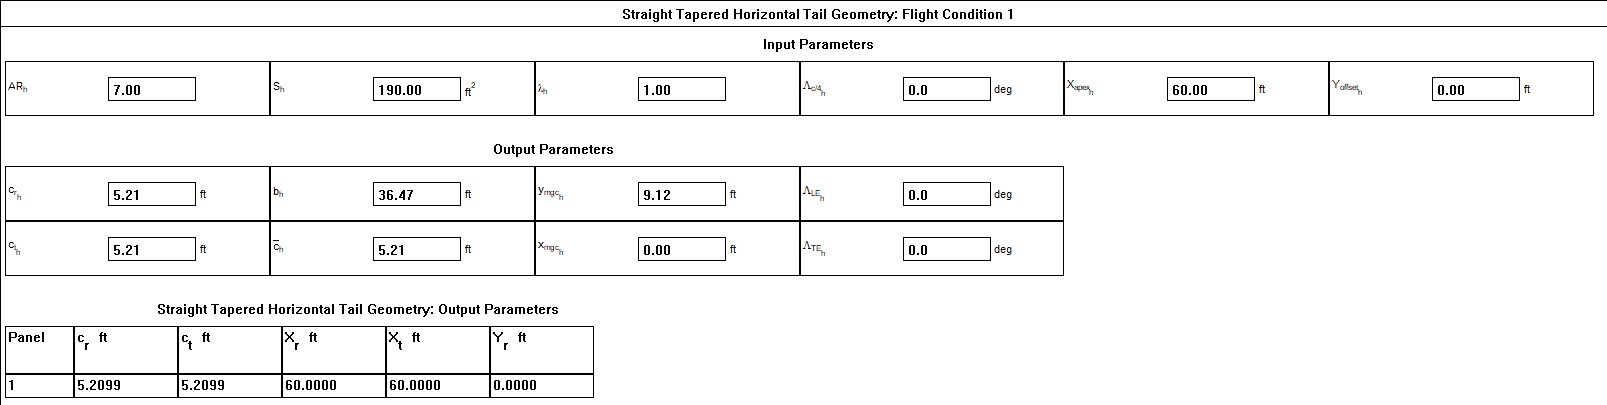
\includegraphics[width=\textwidth]{Report3Printouts/Empannage/Horizontal_geometry_cropped.png}
    \caption{Horizontal stabilizer sizing}
    \label{fig:horizontal_geometry}
\end{figure}

\begin{figure}[H]
    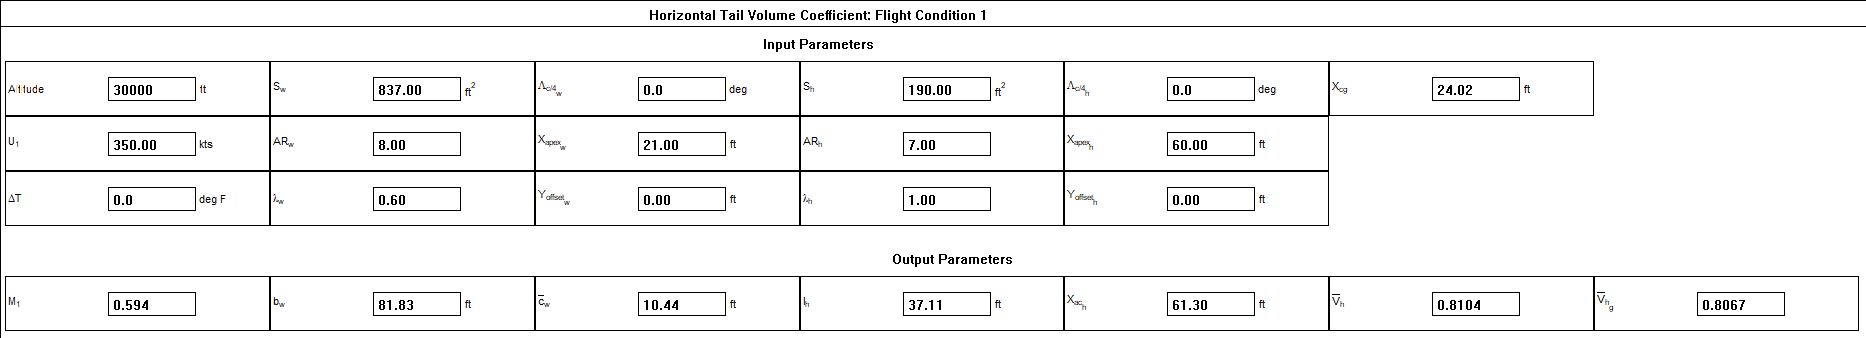
\includegraphics[width=\textwidth]{Report3Printouts/Empannage/Horizontal_volumeratio_cropped.png}
    \caption{Horizontal tail volume coefficient calculations}
    \label{fig:horizontal_volumeratio}
\end{figure}

\begin{figure}[H]
    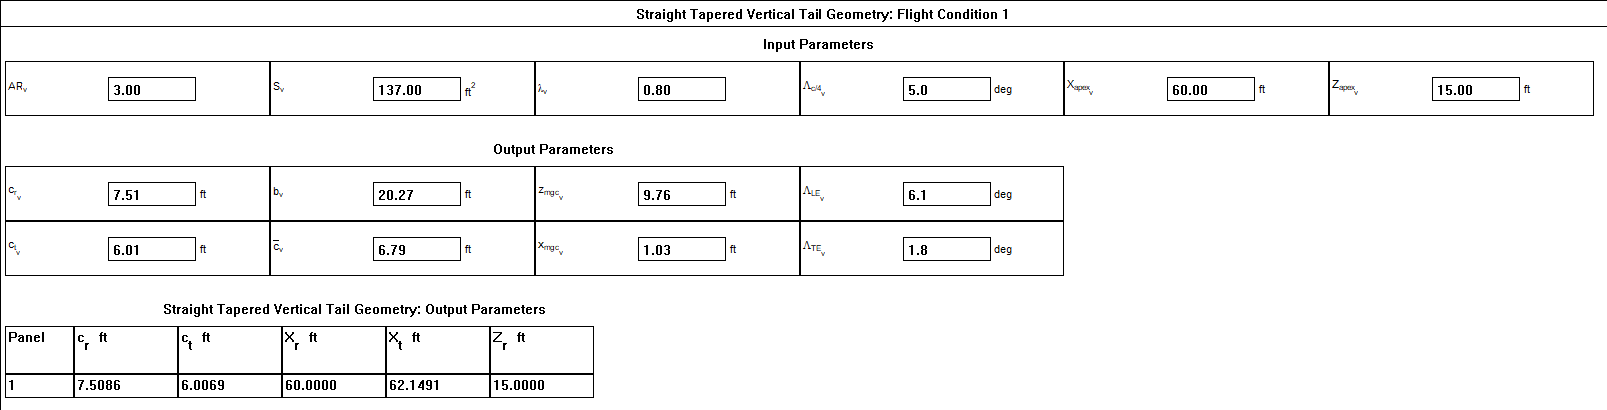
\includegraphics[width=\textwidth]{Report3Printouts/Empannage/Vertical_geometry_cropped.png}
    \caption{Vertical stabilizer sizing}
    \label{fig:vertical_geometry}
\end{figure}

\begin{figure}[H]
    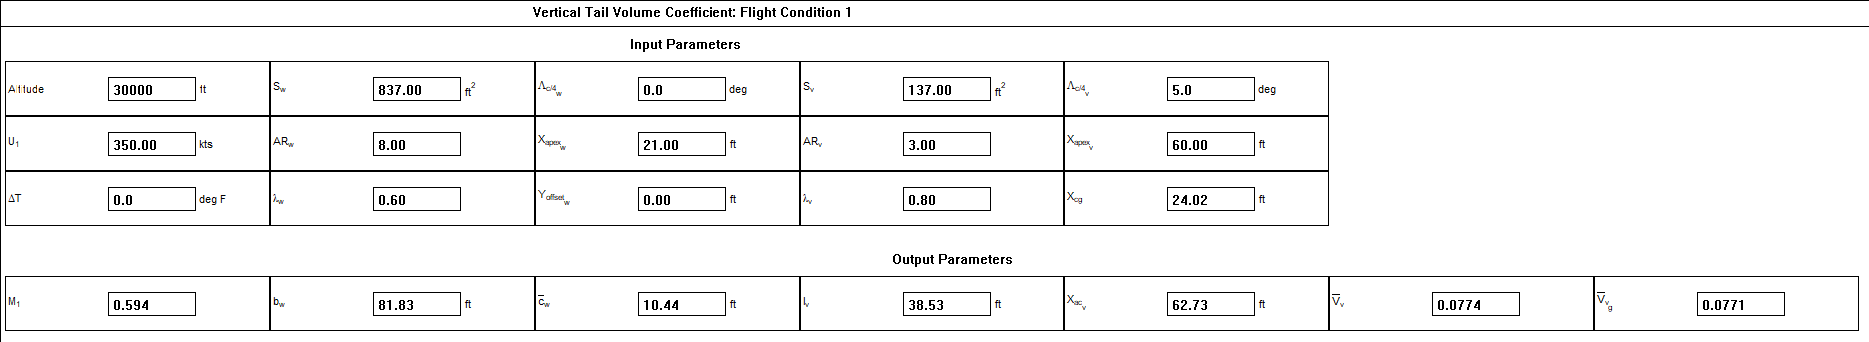
\includegraphics[width=\textwidth]{Report3Printouts/Empannage/Vertical_volumeratio_cropped.png}
    \caption{Vertical stabilizer volume ratio calculation}
    \label{fig:vertical_volumeratio}
\end{figure}

\begin{figure}[H]
    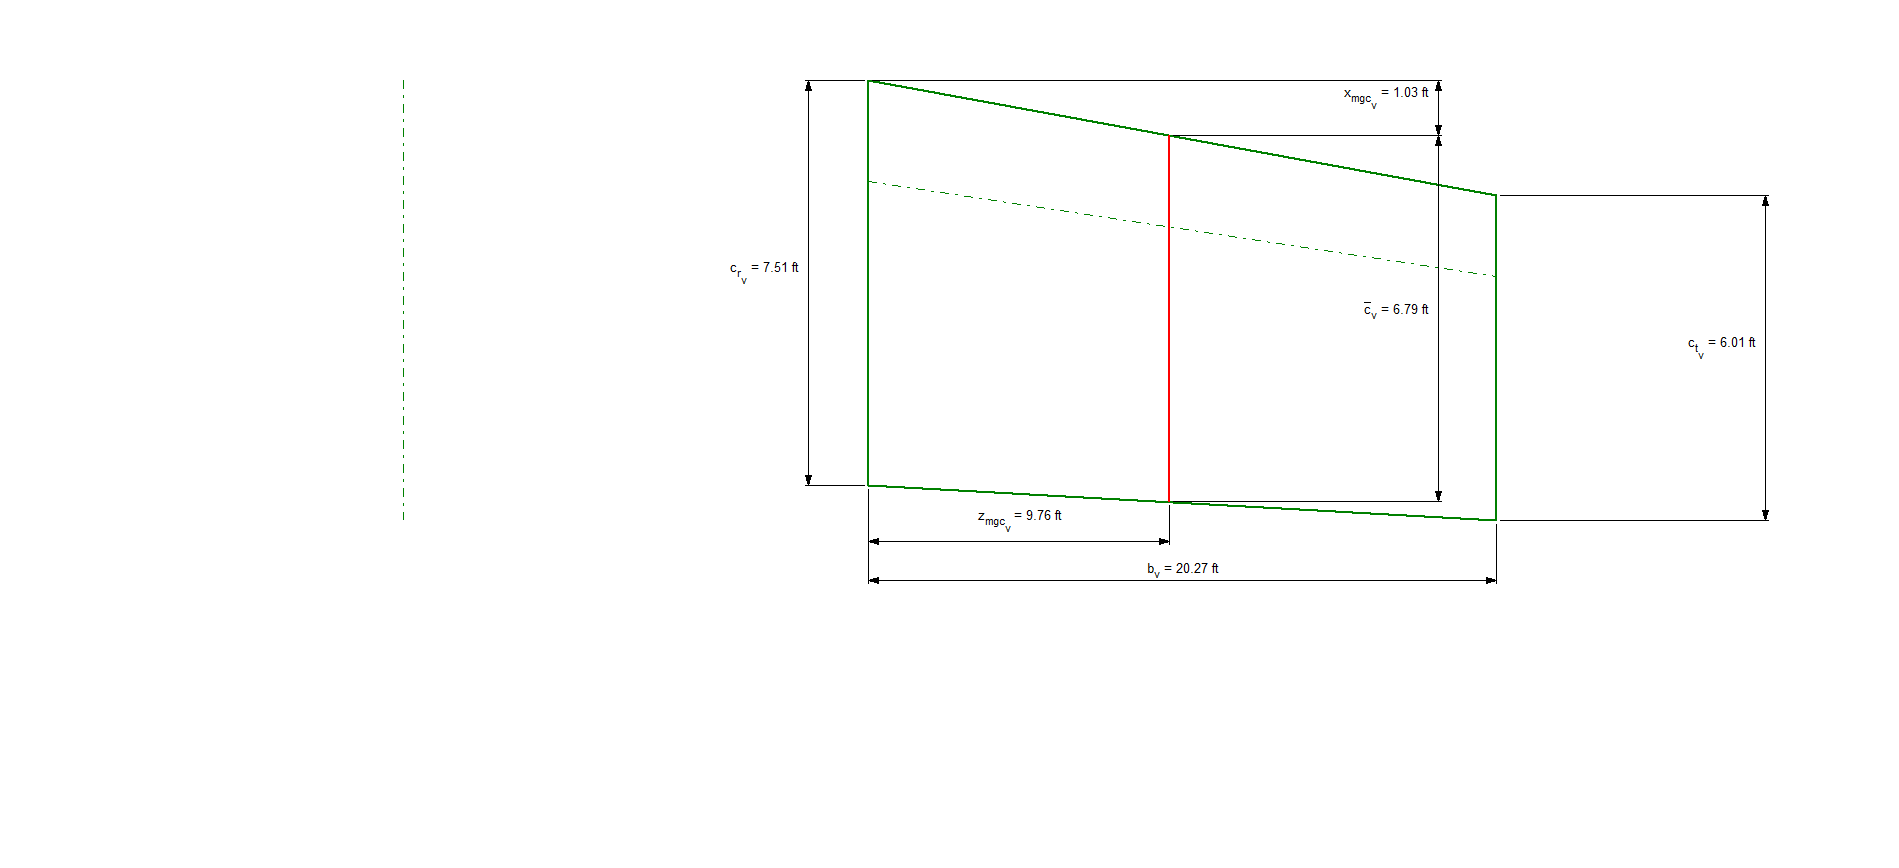
\includegraphics[width=\textwidth]{Report3Printouts/Empannage/Vertical_volumeratio_plot.png}
    \caption{Vertical stabilizer with aerodynamic center shown}
    \label{fig:vertical_volumeratio_plot}
\end{figure}

\begin{figure}[H]
    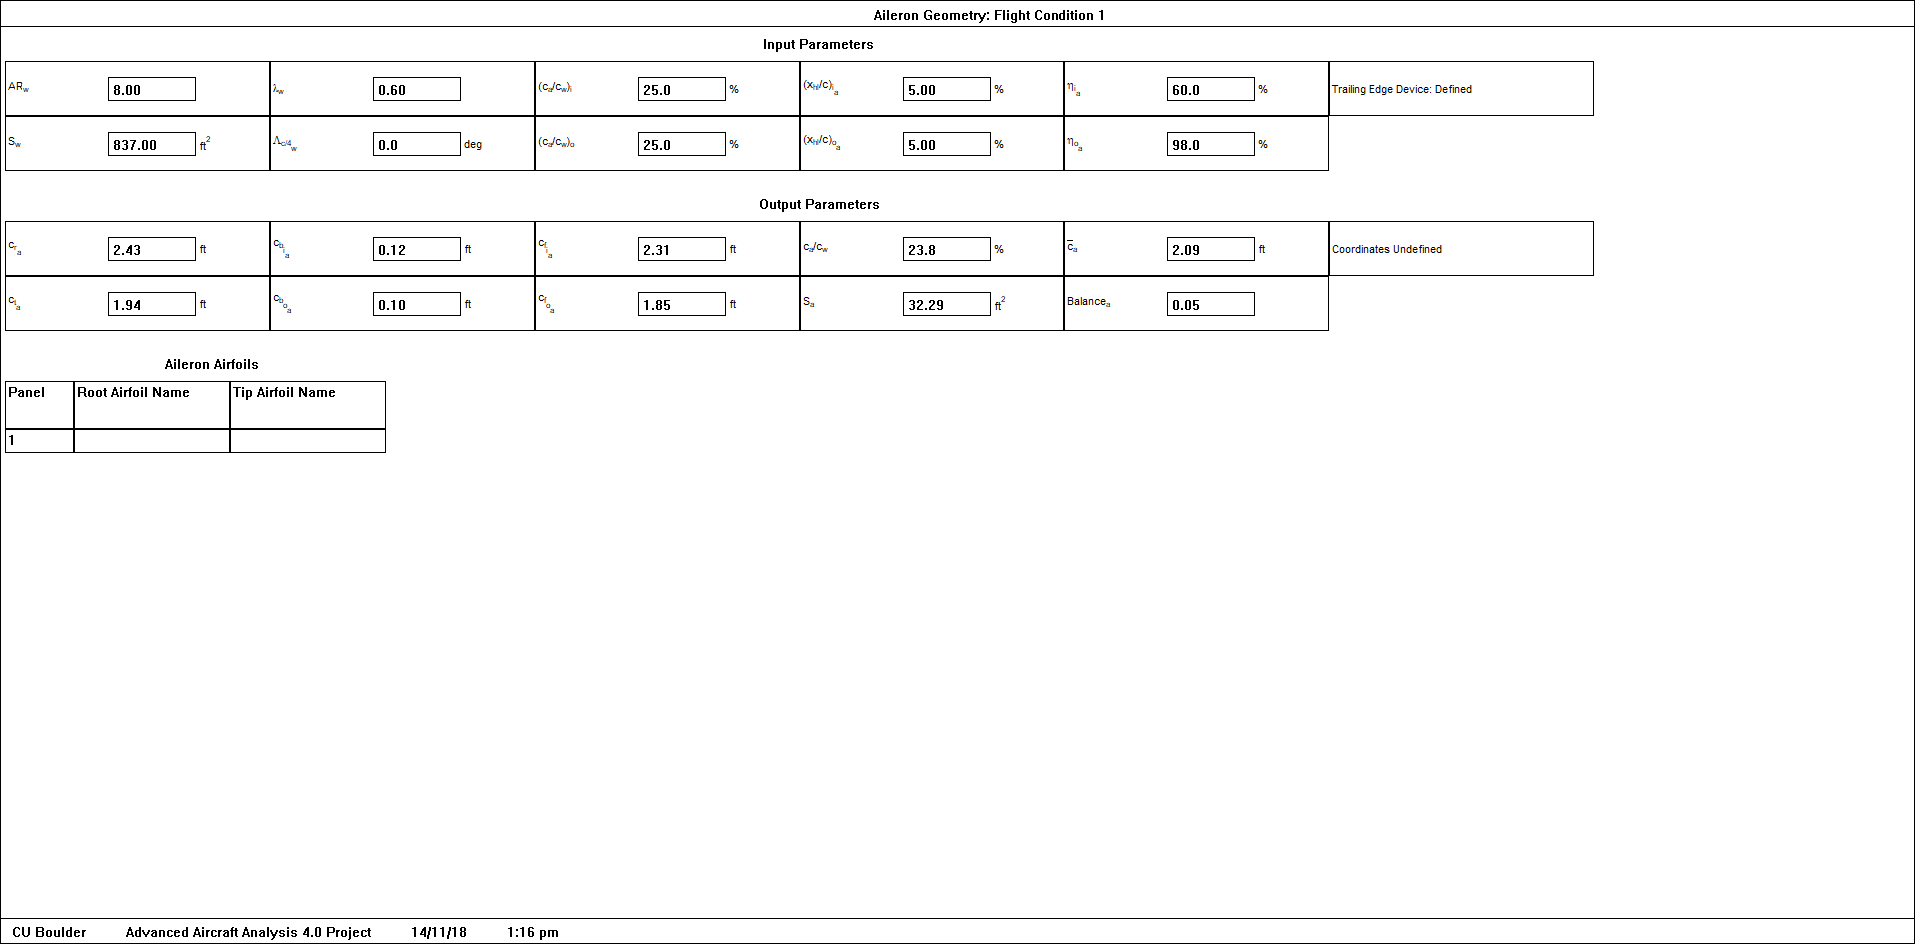
\includegraphics[width=\textwidth]{Report3Printouts/Wing_and_Aileron/aileron_sizing.png}
    \caption{Aileron layout}
    \label{fig:aileron_sizing}
\end{figure}

\subsection{AAA: Control Surface Layout Design}
\begin{figure}[H]
    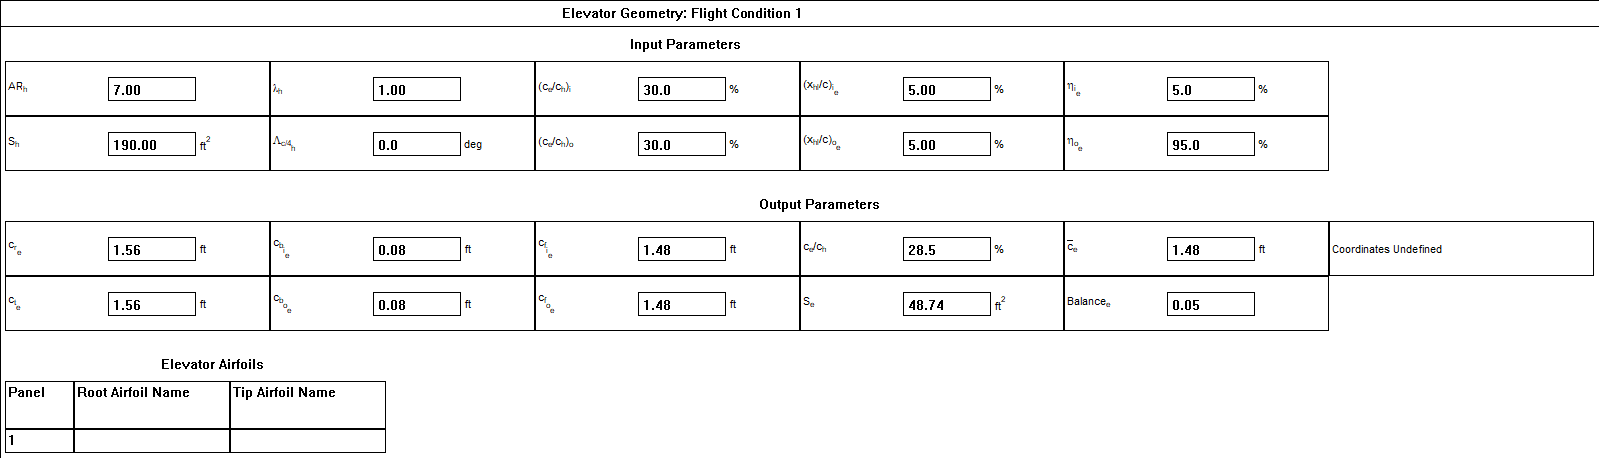
\includegraphics[width=\textwidth]{Report3Printouts/Empannage/Horizontal_elevator_cropped.png}
    \caption{Elevator control surface sizing}
    \label{fig:horizontal_elevator}
\end{figure}

\begin{figure}[H]
    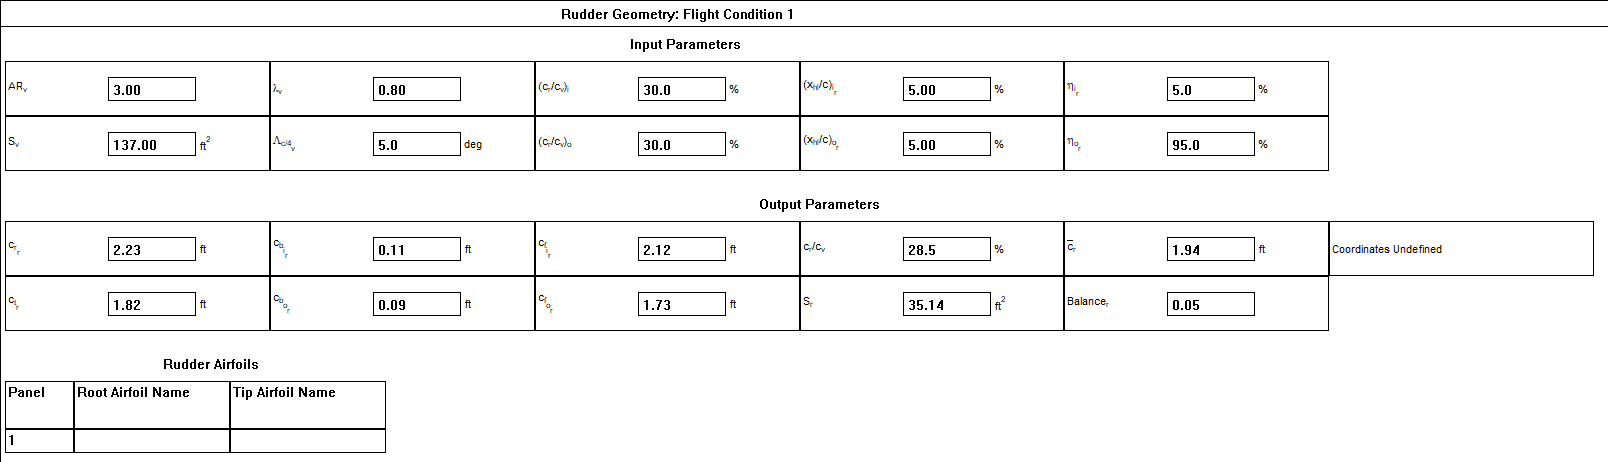
\includegraphics[width=\textwidth]{Report3Printouts/Empannage/Vertical_rudder_cropped.png}
    \caption{Rudder sizing}
    \label{fig:vertical_rudder}
\end{figure}

\subsection{AAA: Stability Derivatives}

\begin{figure}[H]
    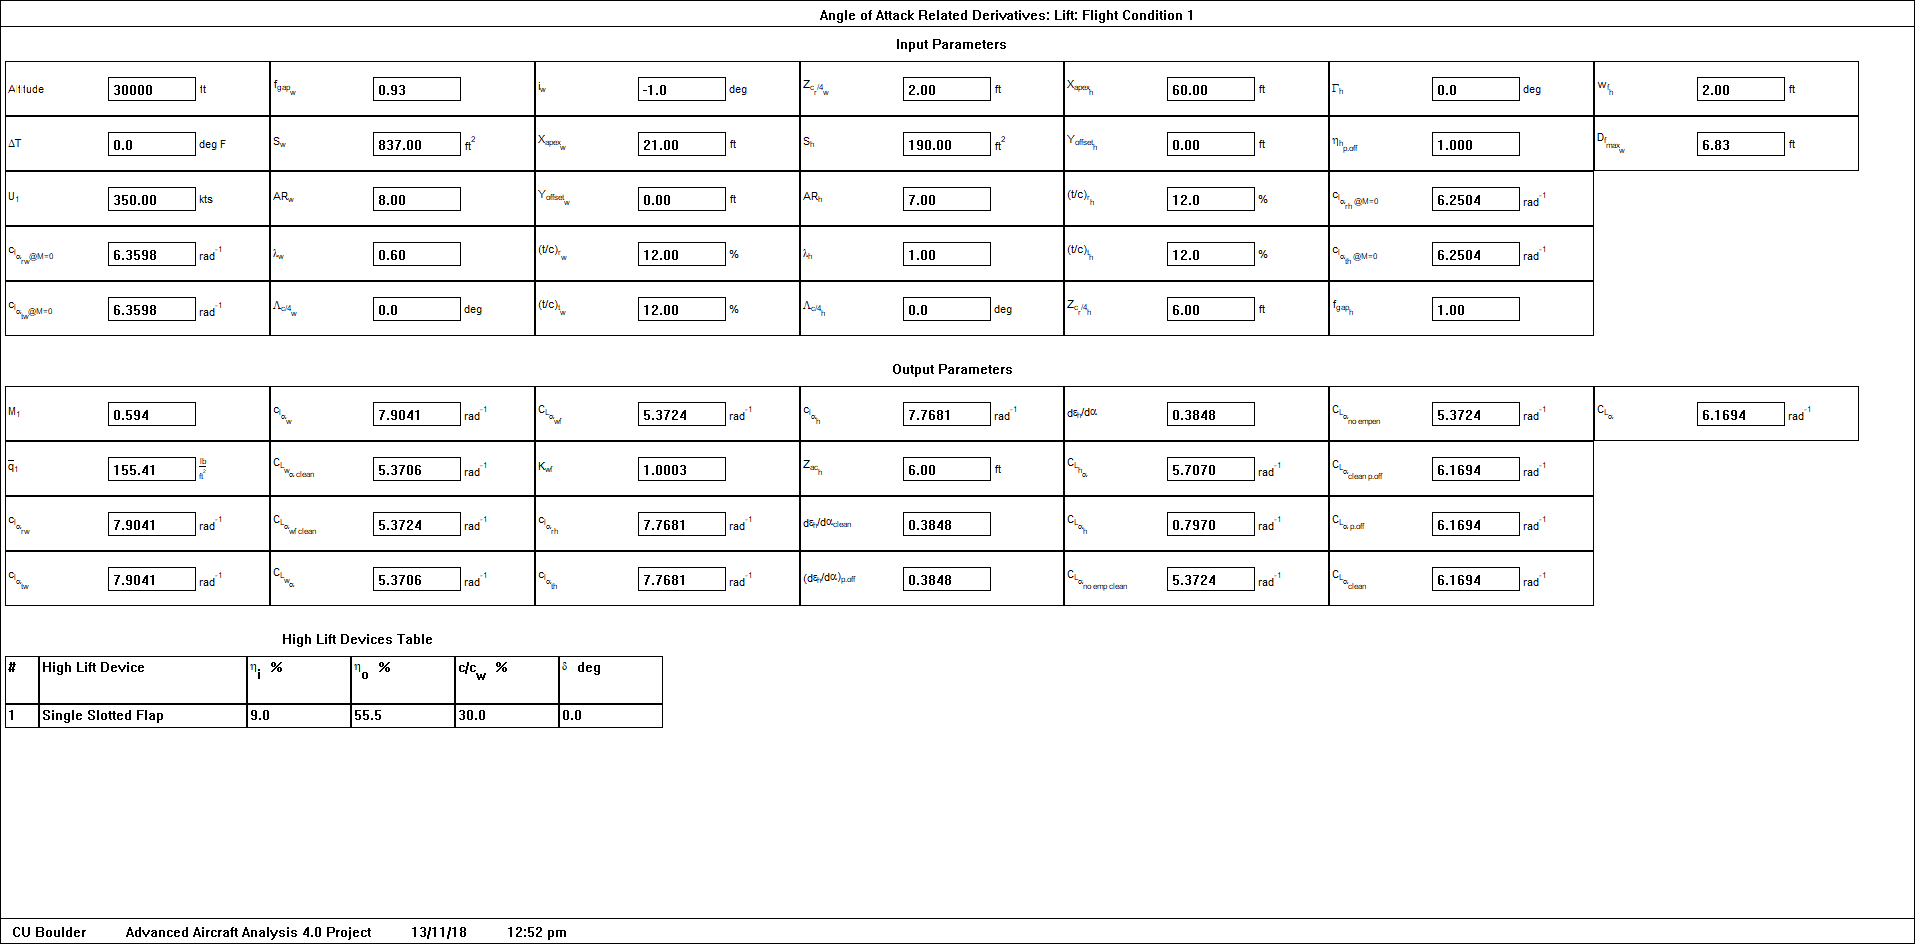
\includegraphics[width=\textwidth]{Report3Printouts/Stability/CL_alpha.png}
    \caption{Calculations of derivatives of $C_L$}
    \label{fig:cl_alpha}
\end{figure}

\begin{figure}[H]
    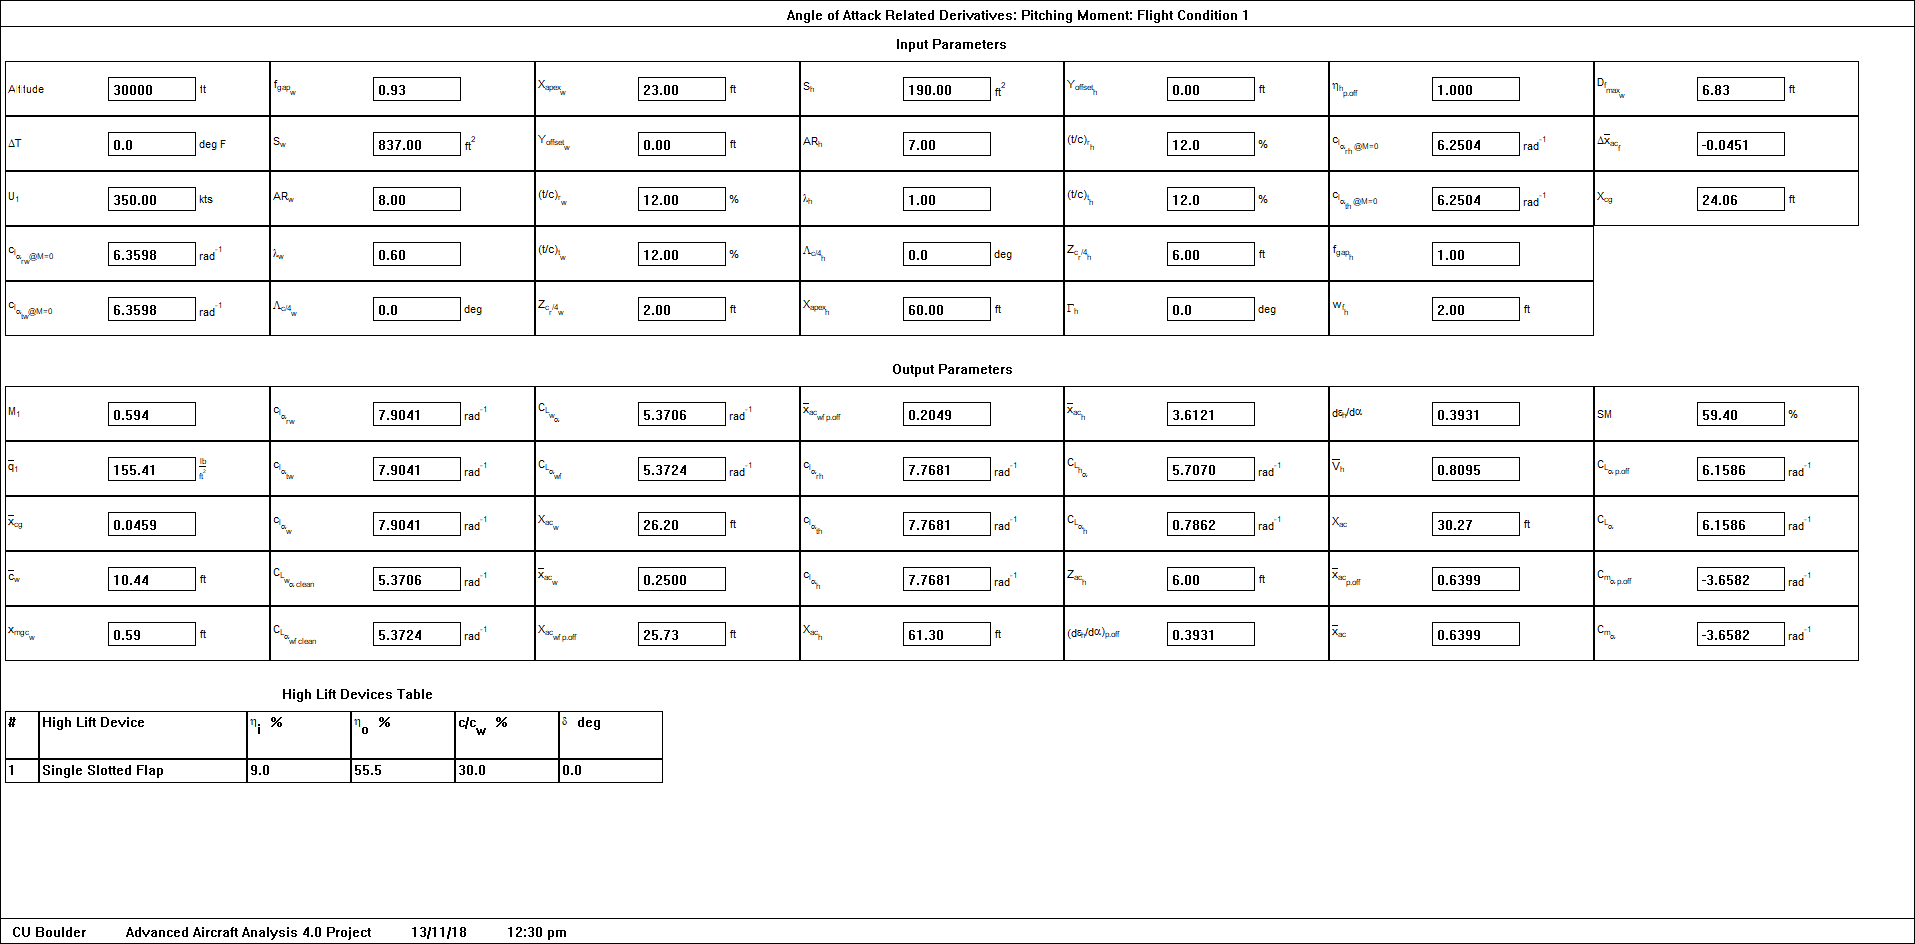
\includegraphics[width=\textwidth]{Report3Printouts/Stability/CM_alpha.png}
    \caption{Initial static margin calculation}
    \label{fig:cm_alpha}
\end{figure}

\begin{figure}[H]
    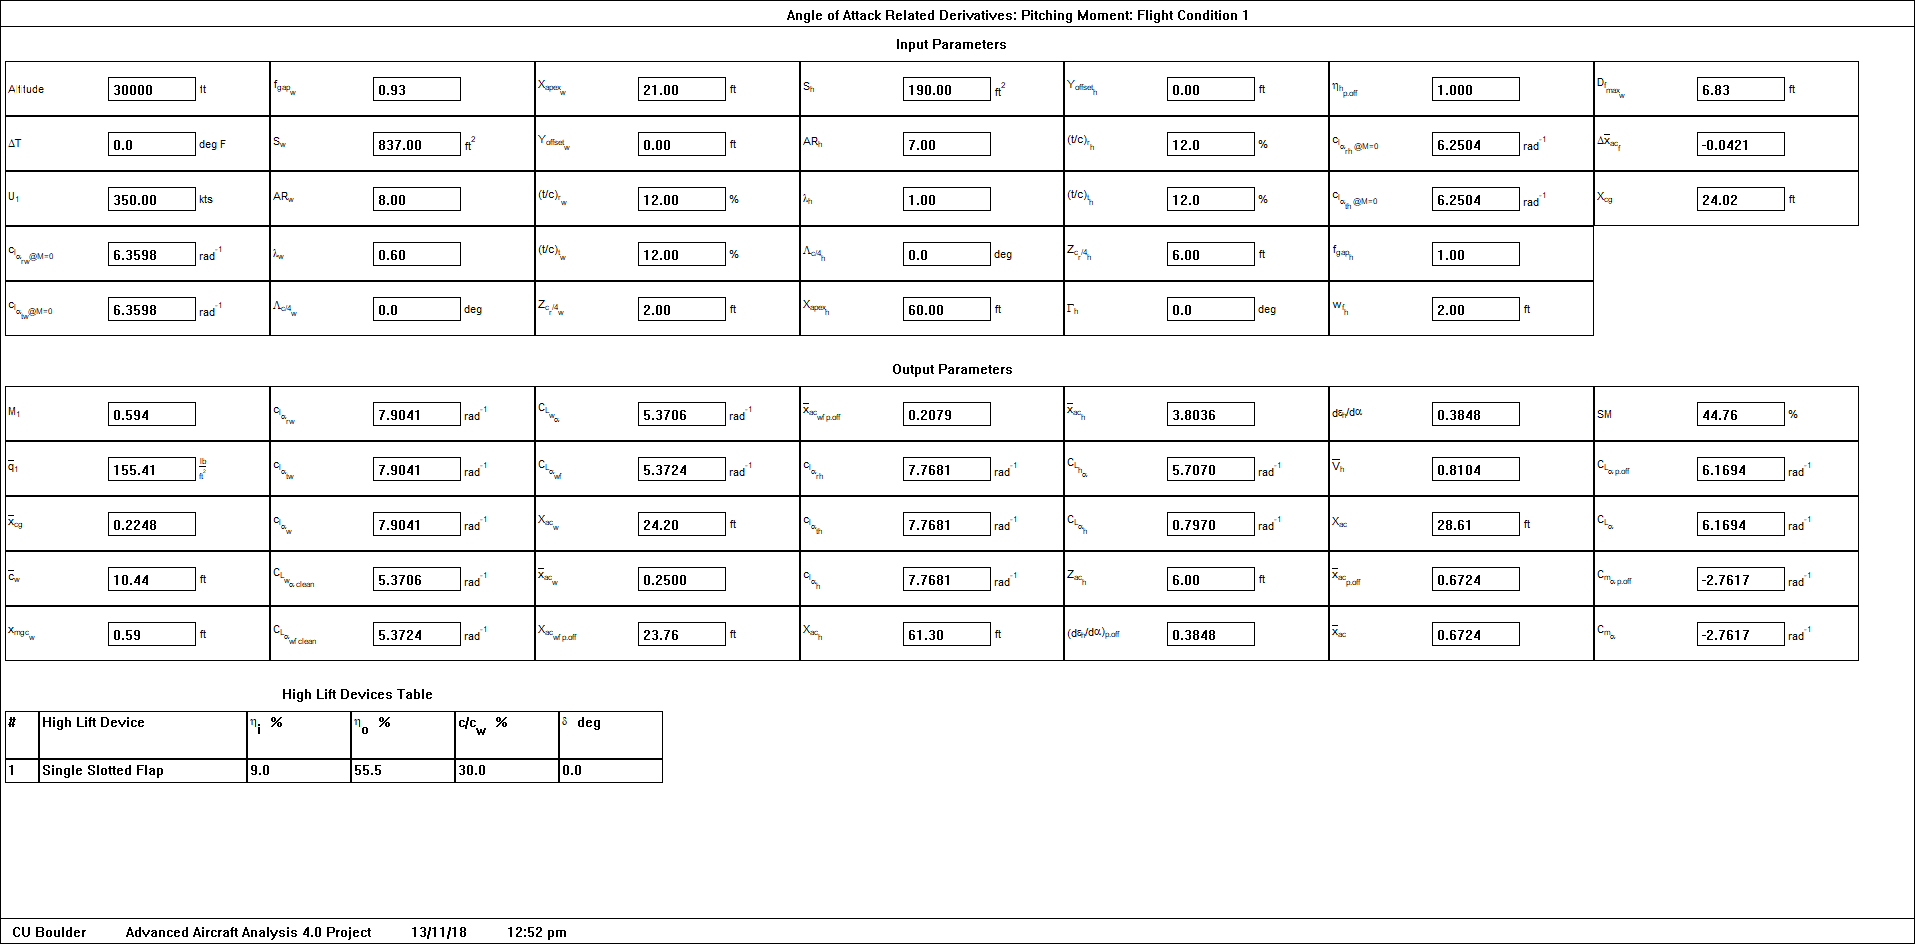
\includegraphics[width=\textwidth]{Report3Printouts/Stability/CM_alpha_final.png}
    \caption{Revised static margin calculation}
    \label{fig:cm_alpha_final}
\end{figure}

\begin{figure}[H]
    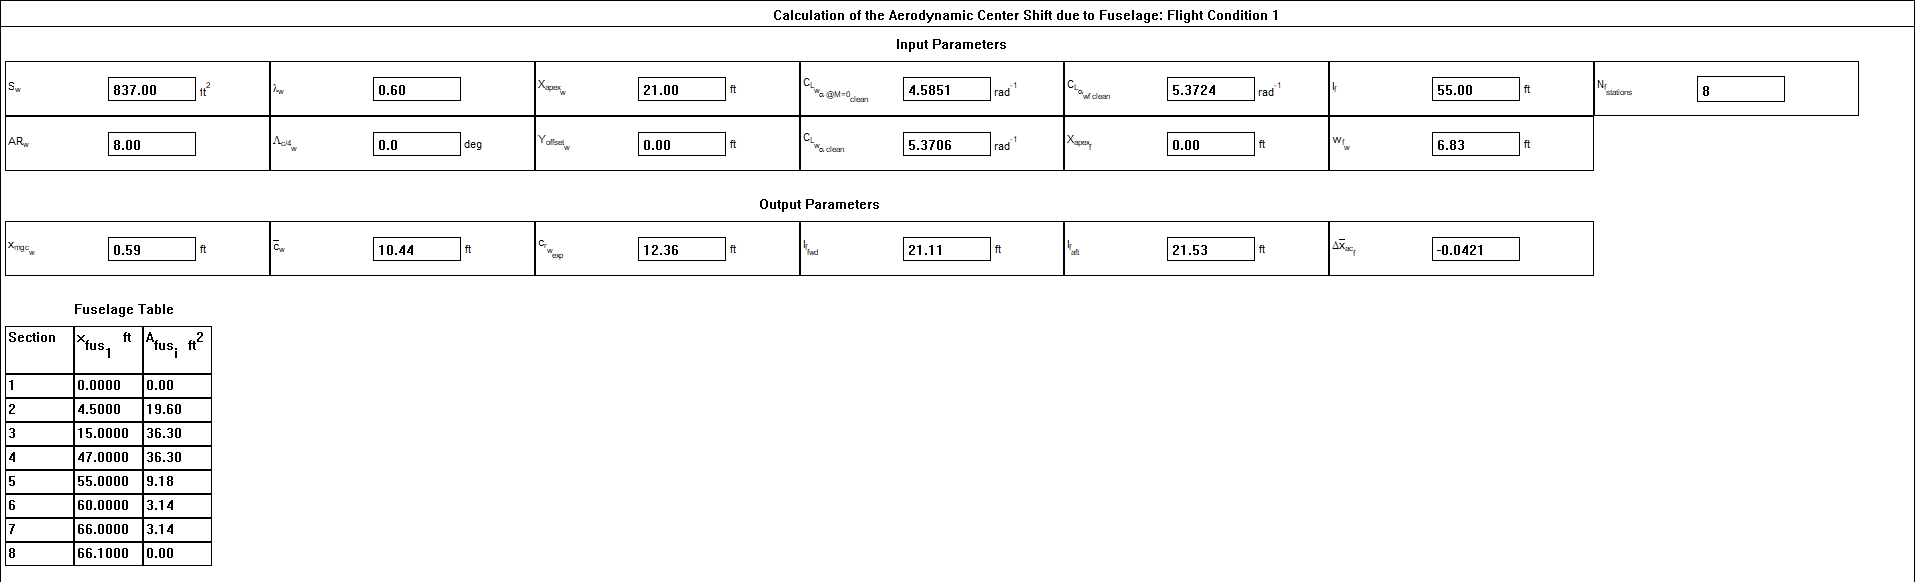
\includegraphics[width=\textwidth]{Report3Printouts/Stability/delta_x_ac_f_cropped.png}
    \caption{Change in aerodynamic center due to fuselage influence}
    \label{fig:delta_x_ac_f}
\end{figure}

\end{document}

